\documentclass[10pt]{article}
%DIF LATEXDIFF DIFFERENCE FILE
%DIF DEL original/Journal_paper/final_sample.tex   Wed Jun 24 12:27:57 2026
%DIF ADD revised/revised_paper_standalone.tex      Wed Jun 24 12:36:49 2026
\usepackage[margin=0.85in]{geometry}
\usepackage{amsmath}
\usepackage{amssymb}
\usepackage{graphicx}
\usepackage{booktabs}
\usepackage{array}
\usepackage{caption}
\usepackage{subcaption}
\usepackage[table]{xcolor}
\usepackage{hyperref}
\usepackage{enumitem}
\usepackage{placeins}
\usepackage{float}
\usepackage{microtype}
\usepackage{subcaption}
\captionsetup[subfigure]{labelformat=empty}
\usepackage{authblk}
\usepackage{titlesec}
\titlespacing*{\section}{0pt}{1.0\baselineskip}{0.4\baselineskip}
\titlespacing*{\subsection}{0pt}{0.7\baselineskip}{0.25\baselineskip}
\titlespacing*{\subsubsection}{0pt}{0.5\baselineskip}{0.2\baselineskip}
\setlength{\textfloatsep}{6pt plus 1pt minus 1pt}
\setlength{\floatsep}{6pt plus 1pt minus 1pt}
\setlength{\intextsep}{6pt plus 1pt minus 1pt}
\setlength{\abovecaptionskip}{2pt}
\setlength{\belowcaptionskip}{0pt}

\hypersetup{
  colorlinks=true,
  linkcolor=blue!55!black,
  citecolor=blue!55!black,
  urlcolor=blue!55!black
}

\captionsetup{font=small, labelfont=bf, skip=4pt}

\title{\textbf{REACH: A Reproducible Benchmark for Rare Malignant Cell
Detection in Single Cell RNA Sequencing}}

\author[1]{Moram Venkata Satya Jaswanth}
\author[1]{Amruthaluri Gavin}
\author[1]{Padarthi Aakash}
\author[1]{Muttha Tejesh Kumar}
\author[1,*]{Abhijit Dasgupta}

\affil[1]{Department of Computer Science and Engineering, SRM University, Andhra Pradesh, India}

\affil[*]{Correspondence: abhijitju06@gmail.com or abhijit.d@srmap.edu.in}
\date{}
%DIF PREAMBLE EXTENSION ADDED BY LATEXDIFF
%DIF UNDERLINE PREAMBLE %DIF PREAMBLE
\RequirePackage[normalem]{ulem} %DIF PREAMBLE
\RequirePackage{color}\definecolor{RED}{rgb}{1,0,0}\definecolor{BLUE}{rgb}{0,0,1} %DIF PREAMBLE
\providecommand{\DIFaddtex}[1]{{\protect\color{trackgreen}#1}} %DIF PREAMBLE
\providecommand{\DIFdeltex}[1]{{\protect\color{red}\sout{#1}}}                      %DIF PREAMBLE
%DIF SAFE PREAMBLE %DIF PREAMBLE
\providecommand{\DIFaddbegin}{} %DIF PREAMBLE
\providecommand{\DIFaddend}{} %DIF PREAMBLE
\providecommand{\DIFdelbegin}{} %DIF PREAMBLE
\providecommand{\DIFdelend}{} %DIF PREAMBLE
\providecommand{\DIFmodbegin}{} %DIF PREAMBLE
\providecommand{\DIFmodend}{} %DIF PREAMBLE
%DIF FLOATSAFE PREAMBLE %DIF PREAMBLE
\providecommand{\DIFaddFL}[1]{\DIFadd{#1}} %DIF PREAMBLE
\providecommand{\DIFdelFL}[1]{\DIFdel{#1}} %DIF PREAMBLE
\providecommand{\DIFaddbeginFL}{} %DIF PREAMBLE
\providecommand{\DIFaddendFL}{} %DIF PREAMBLE
\providecommand{\DIFdelbeginFL}{} %DIF PREAMBLE
\providecommand{\DIFdelendFL}{} %DIF PREAMBLE
%DIF HYPERREF PREAMBLE %DIF PREAMBLE
\providecommand{\DIFadd}[1]{\texorpdfstring{\DIFaddtex{#1}}{#1}} %DIF PREAMBLE
\providecommand{\DIFdel}[1]{\texorpdfstring{\DIFdeltex{#1}}{}} %DIF PREAMBLE
\newcommand{\DIFscaledelfig}{0.5}
%DIF HIGHLIGHTGRAPHICS PREAMBLE %DIF PREAMBLE
\RequirePackage{settobox} %DIF PREAMBLE
\RequirePackage{letltxmacro} %DIF PREAMBLE
\newsavebox{\DIFdelgraphicsbox} %DIF PREAMBLE
\newlength{\DIFdelgraphicswidth} %DIF PREAMBLE
\newlength{\DIFdelgraphicsheight} %DIF PREAMBLE
% store original definition of \includegraphics %DIF PREAMBLE
\LetLtxMacro{\DIFOincludegraphics}{\includegraphics} %DIF PREAMBLE
\newcommand{\DIFaddincludegraphics}[2][]{{\color{trackgreen}\fbox{\DIFOincludegraphics[#1]{#2}}}} %DIF PREAMBLE
\newcommand{\DIFdelincludegraphics}[2][]{% %DIF PREAMBLE
\sbox{\DIFdelgraphicsbox}{\DIFOincludegraphics[#1]{#2}}% %DIF PREAMBLE
\settoboxwidth{\DIFdelgraphicswidth}{\DIFdelgraphicsbox} %DIF PREAMBLE
\settoboxtotalheight{\DIFdelgraphicsheight}{\DIFdelgraphicsbox} %DIF PREAMBLE
\scalebox{\DIFscaledelfig}{% %DIF PREAMBLE
\parbox[b]{\DIFdelgraphicswidth}{\usebox{\DIFdelgraphicsbox}\\[-\baselineskip] \rule{\DIFdelgraphicswidth}{0em}}\llap{\resizebox{\DIFdelgraphicswidth}{\DIFdelgraphicsheight}{% %DIF PREAMBLE
\setlength{\unitlength}{\DIFdelgraphicswidth}% %DIF PREAMBLE
\begin{picture}(1,1)% %DIF PREAMBLE
\thicklines\linethickness{2pt} %DIF PREAMBLE
{\color[rgb]{1,0,0}\put(0,0){\framebox(1,1){}}}% %DIF PREAMBLE
{\color[rgb]{1,0,0}\put(0,0){\line( 1,1){1}}}% %DIF PREAMBLE
{\color[rgb]{1,0,0}\put(0,1){\line(1,-1){1}}}% %DIF PREAMBLE
\end{picture}% %DIF PREAMBLE
}\hspace*{3pt}}} %DIF PREAMBLE
} %DIF PREAMBLE
\LetLtxMacro{\DIFOaddbegin}{\DIFaddbegin} %DIF PREAMBLE
\LetLtxMacro{\DIFOaddend}{\DIFaddend} %DIF PREAMBLE
\LetLtxMacro{\DIFOdelbegin}{\DIFdelbegin} %DIF PREAMBLE
\LetLtxMacro{\DIFOdelend}{\DIFdelend} %DIF PREAMBLE
\DeclareRobustCommand{\DIFaddbegin}{\DIFOaddbegin \let\includegraphics\DIFaddincludegraphics} %DIF PREAMBLE
\DeclareRobustCommand{\DIFaddend}{\DIFOaddend \let\includegraphics\DIFOincludegraphics} %DIF PREAMBLE
\DeclareRobustCommand{\DIFdelbegin}{\DIFOdelbegin \let\includegraphics\DIFdelincludegraphics} %DIF PREAMBLE
\DeclareRobustCommand{\DIFdelend}{\DIFOaddend \let\includegraphics\DIFOincludegraphics} %DIF PREAMBLE
\LetLtxMacro{\DIFOaddbeginFL}{\DIFaddbeginFL} %DIF PREAMBLE
\LetLtxMacro{\DIFOaddendFL}{\DIFaddendFL} %DIF PREAMBLE
\LetLtxMacro{\DIFOdelbeginFL}{\DIFdelbeginFL} %DIF PREAMBLE
\LetLtxMacro{\DIFOdelendFL}{\DIFdelendFL} %DIF PREAMBLE
\DeclareRobustCommand{\DIFaddbeginFL}{\DIFOaddbeginFL \let\includegraphics\DIFaddincludegraphics} %DIF PREAMBLE
\DeclareRobustCommand{\DIFaddendFL}{\DIFOaddendFL \let\includegraphics\DIFOincludegraphics} %DIF PREAMBLE
\DeclareRobustCommand{\DIFdelbeginFL}{\DIFOdelbeginFL \let\includegraphics\DIFdelincludegraphics} %DIF PREAMBLE
\DeclareRobustCommand{\DIFdelendFL}{\DIFOaddendFL \let\includegraphics\DIFOincludegraphics} %DIF PREAMBLE
%DIF COLORLISTINGS PREAMBLE %DIF PREAMBLE
\RequirePackage{listings} %DIF PREAMBLE
\RequirePackage{color} %DIF PREAMBLE
\lstdefinelanguage{DIFcode}{ %DIF PREAMBLE
%DIF DIFCODE_UNDERLINE %DIF PREAMBLE
  moredelim=[il][\color{red}\sout]{\%DIF\ <\ }, %DIF PREAMBLE
  moredelim=[il][\color{blue}\uwave]{\%DIF\ >\ } %DIF PREAMBLE
} %DIF PREAMBLE
\lstdefinestyle{DIFverbatimstyle}{ %DIF PREAMBLE
	language=DIFcode, %DIF PREAMBLE
	basicstyle=\ttfamily, %DIF PREAMBLE
	columns=fullflexible, %DIF PREAMBLE
	keepspaces=true %DIF PREAMBLE
} %DIF PREAMBLE
\lstnewenvironment{DIFverbatim}{\lstset{style=DIFverbatimstyle}}{} %DIF PREAMBLE
\lstnewenvironment{DIFverbatim*}{\lstset{style=DIFverbatimstyle,showspaces=true}}{} %DIF PREAMBLE
%DIF END PREAMBLE EXTENSION ADDED BY LATEXDIFF

\providecommand{\tightlist}{\setlength{\itemsep}{0pt}\setlength{\parskip}{0pt}}
\definecolor{trackgreen}{RGB}{0,150,0}
\begin{document}
\maketitle

%DIF <  -----------ABSTRACT---------
\DIFdelbegin %DIFDELCMD < \begin{abstract}
%DIFDELCMD < \noindent
%DIFDELCMD < %%%
\DIFdelend \DIFaddbegin \section{\DIFadd{REACH: A Reproducible Benchmark for Rare Malignant-Cell
Detection in Single-Cell RNA
Sequencing}}\label{reach-a-reproducible-benchmark-for-rare-malignant-cell-detection-in-single-cell-rna-sequencing}

\begin{quote}
\textbf{\DIFadd{Article type:}} \DIFadd{Original Research \textbar{} }\textbf{\DIFadd{Version:}}
\DIFadd{v1.2.0 \textbar{} }\textbf{\DIFadd{Date:}} \DIFadd{2026-04-30
}\end{quote}

\begin{center}\DIFadd{\rule{0.5\linewidth}{0.5pt}}\end{center}

\subsection{\DIFadd{Abstract}}\label{abstract}

\DIFaddend Rare malignant cells in \DIFdelbegin \DIFdel{single cell }\DIFdelend \DIFaddbegin \DIFadd{single-cell }\DIFaddend RNA sequencing (scRNA-seq) \DIFdelbegin \DIFdel{span
}\DIFdelend \DIFaddbegin \DIFadd{can
represent }\DIFaddend circulating tumor cells, \DIFaddbegin \DIFadd{minimal }\DIFaddend residual disease,
\DIFdelbegin \DIFdel{drug tolerant persisters, and
small malignant }\DIFdelend \DIFaddbegin \DIFadd{drug-tolerant persisters, metastatic intermediates, or small tumor
}\DIFaddend compartments embedded in \DIFdelbegin \DIFdel{heterogeneous tumor
microenvironments. To detect rare cells , existing methods have been evaluated inconsistently because
studies differ in datasets, label definitions, prevalence regimes, score
contracts, and failure handling.
Here, we present }\DIFdelend \DIFaddbegin \DIFadd{a complex microenvironment. REACH targets the
specific problem of }\textbf{\DIFadd{rare malignant-cell detection in a
heterogeneous tumour microenvironment (TME)}}\DIFadd{: positives are malignant
cells embedded in an immune/stromal background, and the task is
}\textbf{\DIFadd{imbalanced cell-level ranking}}\DIFadd{, not intra-lineage sub-state
discovery. REACH therefore evaluates how well methods surface scarce
malignant cells above an abundant TME background under controlled
prevalence, synthetic stress, null-control, and label-noise conditions.
These populations are biologically important but statistically
difficult: the positive class is scarce, labels are assembled from
imperfect evidence, and a high AUROC can coexist with poor recovery of
top-ranked cells. We present REACH, not a new detector but }\DIFaddend a
reproducible benchmark \DIFdelbegin \DIFdel{framework,  Rare cell Evaluation Across Cancer Heterogeneity (REACH),  that treats rare
malignant cell detection as an
imbalanced ranking task. REACH combines confidence tiered multi arm labels,five complementary }\DIFdelend \DIFaddbegin \DIFadd{and software/data resource for rare
malignant-cell detection that treats the task as imbalanced cell-level
ranking. REACH v1.2.0 combines ten curated public scRNA-seq datasets
(approx. 360,000 cells), six }\DIFaddend evaluation tracks (\DIFdelbegin \DIFdel{controlled real spike-ins, synthetic
splatter stress, null background controls, natural blood/CTC prevalence, and
supervised label noise diagnostics), }\DIFdelend \DIFaddbegin \DIFadd{A--F), ten }\DIFaddend standardized
method wrappers, \DIFdelbegin \DIFdel{fallback aware
}\DIFdelend \DIFaddbegin \DIFadd{confidence-tiered multi-arm labels, fallback-aware
}\DIFaddend metrics, nonparametric \DIFaddbegin \DIFadd{paired }\DIFaddend statistics, and figure regeneration from
\DIFdelbegin \DIFdel{audited
}\DIFdelend \DIFaddbegin \DIFadd{frozen }\DIFaddend result tables. \DIFdelbegin \DIFdel{In its current form, REACH evaluates ten recent computational methods on ten curated scRNA-seq cancer datasets comprising 359,739 cells. }\DIFdelend Across 1,\DIFdelbegin \DIFdel{110 benchmark tasks, this produces }\DIFdelend \DIFaddbegin \DIFadd{125 benchmark units, REACH produced
}\DIFaddend 11,\DIFdelbegin \DIFdel{100 individual method performance measurements. The supervised highly variable gene logistic regression ceiling
achieves near perfect separation for many tumor related labels, with a }\DIFdelend \DIFaddbegin \DIFadd{250 method-unit evaluations. On the primary controlled real-cell
Track A endpoint, the supervised in-sample }\texttt{\DIFadd{hvg\_logreg}} \DIFadd{ceiling
reached }\DIFaddend median average precision \DIFdelbegin \DIFdel{of 1.0, indicating clear gene expression differences between tumor related and non tumor cell populations. In contrast, current unsupervised ranking methods recover only part of these differences}\DIFdelend \DIFaddbegin \DIFadd{(AP) 1.000 (mean 0.909, mean AUROC
0.953), showing that high-confidence labels often retain recoverable
expression signal}\DIFaddend . The exploratory comparator \DIFdelbegin \DIFdel{CaSee obtains a median average precision of }\DIFdelend \DIFaddbegin \texttt{\DIFadd{CaSee}} \DIFadd{reached
median AP }\DIFaddend 0.512 \DIFdelbegin \DIFdel{, whereas FiRE, the strongest ranked published
detector, achieves a median average precision of }\DIFdelend \DIFaddbegin \DIFadd{but is reported separately from ranked published
detectors. Among ranked published methods, }\texttt{\DIFadd{FiRE}} \DIFadd{had the highest
primary median AP (}\DIFaddend 0.313\DIFdelbegin \DIFdel{. Statistical testing confirms substantial performance differences among methods on the common benchmark subset . More importantly, REACH shows that performance is highly context dependent: no single method consistently performs best across tumor types, and method behavior under ranking,
null controls, and label noise cannot be adequately represented by a single summary score. These findings highlight a
clear }\DIFdelend \DIFaddbegin \DIFadd{), while paired tests showed it was not
significantly different from }\texttt{\DIFadd{expr\_threshold}} \DIFadd{or
}\texttt{\DIFadd{scMalignantFinder}}\DIFadd{. Global Track A method differences were
strongly supported on the 140-unit common subset (Friedman χ²=695.05,
p=8.0×10⁻¹⁴⁴; Iman-Davenport F=171.01, p=8.4×10⁻²¹¹). REACH exposes a
large }\DIFaddend gap between supervised \DIFdelbegin \DIFdel{expression-based separability and the current performance of unsupervised
rare malignant cell detection methods. All code, data, figures,
and documentation required to reproduce the analysis are available in the public GitHub repository: }%DIFDELCMD < \url{https://github.com/jaswanthmoram/reach-rarecell-benchmark}
%DIFDELCMD < \end{abstract}
%DIFDELCMD < 

%DIFDELCMD < %%%
%DIF <  ------------INTRODUCTION SECTION 1----------
\section{\DIFdel{Introduction}}
%DIFAUXCMD
\addtocounter{section}{-1}%DIFAUXCMD
%DIFDELCMD < 

%DIFDELCMD < %%%
\DIFdel{Tumor samples are often highly mixed. Along with dominant malignant and non-malignant populations, they may contain small groups of cells that are biologically important but difficult to observe in bulk measurements. Single-cell RNA sequencing (scRNA-seq) allows us to look at such populations of cells separately, and to investigate tumor heterogeneity with an unprecedented level of detail \mbox{%DIFAUXCMD
\cite{papalexi2018single,tirosh2024cancer}}\hskip0pt%DIFAUXCMD
. This is especially important when it comes to circulating tumor cells, metastatic intermediates, minimal residual disease cells, drug-tolerant persisters and small malignant compartments in the tumor microenvironment. These populations can be low-frequency, }\textit{\DIFdel{e.g.}}%DIFAUXCMD
\DIFdel{, contribute to 1\% or less in a given dataset \mbox{%DIFAUXCMD
\cite{torre2018rare,gao2021delineating}}\hskip0pt%DIFAUXCMD
. That not only makes them challenging to identify in biological terms, but also in statistical ones. They can be more difficult to extract if rare cells are in a more diluted cluster. If these cells are rare, mixed with neighbouring cells expressing related cell-types or have low confidence from expression and copy numberevidence, they become nearly impossible to identify \mbox{%DIFAUXCMD
\cite{martens2023rarity,stegle2015computational,ren2018understanding}}\hskip0pt%DIFAUXCMD
}\DIFdelend \DIFaddbegin \DIFadd{separability and current unsupervised
ranking, substantial prevalence sensitivity, dataset-specific winners,
and method reliability issues that would be hidden by a single
leaderboard number}\DIFaddend .

\DIFdelbegin \DIFdel{This is particularly challenging for cancer data sets where the label malignant may not be clear-cut. A cell can be classified as malignant based on copy number alteration, cancer associated expression signatures, somatic mutation evidence, neighborhood structure or expert annotations \mbox{%DIFAUXCMD
\cite{gao2021delineating,gasper2022variant,nofech2023pan}}\hskip0pt%DIFAUXCMD
. However, in practice, the evidential sources may not be fully congruent. For some cells, there is strong evidence of expression but weak support by copy number, while others can be hard to classify if they are near non malignant populations. This sets rare malignant cell detection apart from its cousin cell-type annotation, where the expected classes are usually more clearly delineated. Moreover, the problem is extremely imbalanced as there are frequently many more background cells surrounding the malignant cells of interest \mbox{%DIFAUXCMD
\cite{johnson2019survey,altalhan2025imbalanced}}\hskip0pt%DIFAUXCMD
.
}%DIFDELCMD < 

%DIFDELCMD < %%%
\DIFdel{This imbalance also raises questions about how methods should be assessed. The Area Under the Receiver Operating Characteristic Curve (AUROC) is widely used as a performance metric for machine learning classification and ranking tasks, but it becomes unwieldy and confusing if the positive class size shrinks very small. If true rare malignant cells are not ranked anywhere near the top of the list for a method, it may obtain a quite reasonable AUROC. Due to the high imbalance ratio, precision recall based measures are often more meaningful in this setting since they reflect whether rare positive cells are recovered among the highest ranked predictions \mbox{%DIFAUXCMD
\cite{davis2006relationship,saito2015precision}}\hskip0pt%DIFAUXCMD
. However, performance should never be evaluated on just a single statistic. Changing label definition, data distribution, null behavior, method failure and statistical error makes how to interpret benchmark results a complex matter.
}%DIFDELCMD < 

%DIFDELCMD < %%%
\DIFdel{There have been multiple scRNA-seq benchmarks that have already been created to test batch effect correction, clustering, cell-type annotation and rare cell discovery. These benchmarks serve as useful reference standards for method comparison. Nevertheless, rare malignant-cell detection requires a more tailored assessment plan. The targeted population may be very small, the label may require multiple types of biological evidence, and the same approach may not perform uniformly across tumor types, sequencing platforms or prevalence settings \mbox{%DIFAUXCMD
\cite{tran2020benchmark,wang2022comparison,tian2019benchmarking,abdelaal2019comparison}}\hskip0pt%DIFAUXCMD
. Thus, a benchmark for this task should not return just one best method. It should use common rules to compare methods, separate supervised reference performance from unsupervised ranking performance, log failed or unstable runs, include null control analysis, and report results in a cancer and dataset specific manner\mbox{%DIFAUXCMD
\cite{cao2021benchmark}}\hskip0pt%DIFAUXCMD
.
}\DIFdelend \DIFaddbegin \begin{center}\DIFadd{\rule{0.5\linewidth}{0.5pt}}\end{center}
\DIFaddend 

\DIFdelbegin \DIFdel{We herein present }\textit{\DIFdel{Rare cell Evaluation Across Cancer Heterogeneity}} %DIFAUXCMD
\DIFdel{(REACH), a reproducible benchmark for rare malignant cell detection in scRNA-seq data (Fig. ~\ref{fig:pipeline}). REACH formulates the detection of rare malignant cells as an imbalanced ranking problem. It is to expect that a method would give more scores to high-confidence malignant cells than to high confidence background cells. It contains the various stages of a typical pipeline, from data ingestion and preprocessing to multi evidence label construction, evaluation track generation, method execution, metric summarization and statistical analysis.
}\DIFdelend \DIFaddbegin \subsection{\DIFadd{Public Release Scope}}\label{public-release-scope}
\DIFaddend 

\DIFdelbegin \DIFdel{Five evaluation tracks were designed to analyze different aspects of method behavior in REACH (Fig. ~\ref{fig:tracks}). Track A evaluates real malignant cells under controlled rarity levels and serves as the primary ranking endpoint. Track B tests method performance under synthetic stress. Track C uses background-dominated controls to assess false-positive behavior when rare malignant cells are not expected. Track D evaluates natural prevalence in blood and circulating tumor cell datasets. Track E examines how the supervised ceiling changes when labels are deliberately corrupted; therefore, it is interpreted as a supervised label noise diagnostic rather than as a general robustness test for unsupervised methods. The current audited REACH snapshot includes 10 datasets, 10 methods, and }\DIFdelend \DIFaddbegin \DIFadd{This repository contains source code, tests, method wrappers, workflow
entrypoints, toy data, lightweight Phase }\DIFaddend 11 \DIFdelbegin \DIFdel{,100 individual method performance measurements. The framework also provides instructions for adding new datasets and methods, so that it can be extended in future studies.
}%DIFDELCMD < 

%DIFDELCMD < %%%
\DIFdel{The results show that many high confidence malignant and
  background labels contain gene-expression differences that can be recovered by a supervised model. However, current unsupervised and rarity-based methods recover only part of this separation on the primary Track A endpoint \mbox{%DIFAUXCMD
\cite{abdelaal2019comparison,mahalanabis2022evaluation}}\hskip0pt%DIFAUXCMD
. REACH also shows that method performance changes across datasets and evaluation tracks. A method that performs well in one tumor context may not remain the strongest method in another \mbox{%DIFAUXCMD
\cite{xu2024sccad,ye2025revealing}}\hskip0pt%DIFAUXCMD
. These findings support the need for a reproducible benchmark that evaluates rare malignant-cell detection in relation to dataset context, rarity level, failure behavior, and evaluation condition.
}\DIFdelend \DIFaddbegin \DIFadd{CSV snapshots, Phase 12 PNG
previews, and submission-ready figures. Large processed datasets, track
units, full prediction outputs, and complete result archives are
external Zenodo/GitHub release assets.
}\DIFaddend 

%DIF <  --------------RELATED WORK SECTION 2----------
\DIFdelbegin \section{\DIFdel{Related work}}
%DIFAUXCMD
\addtocounter{section}{-1}%DIFAUXCMD
\DIFdelend \DIFaddbegin \begin{center}\DIFadd{\rule{0.5\linewidth}{0.5pt}}\end{center}
\DIFaddend 

\DIFdelbegin \subsection{\DIFdel{Rare cell discovery in scRNA-seq}}
%DIFAUXCMD
\addtocounter{subsection}{-1}%DIFAUXCMD
\DIFdelend \DIFaddbegin \subsection{\DIFadd{Contributions}}\label{contributions}
\DIFaddend 

\DIFdelbegin \DIFdel{Finder of Rare Entities (FiRE) assigns a density-derived rarity score to each cell and is included in REACH as one of the ranked published comparators \mbox{%DIFAUXCMD
\cite{martens2023rarity}}\hskip0pt%DIFAUXCMD
. The Cell Subtype Identification from Up regulated gene Sets (CellSIUS) method uses up regulated gene sets and greater specificity for rare sub populations of complex single cell populations from single cell RNA sequencing to detect rare populations \mbox{%DIFAUXCMD
\cite{wegmann2019cellsius}}\hskip0pt%DIFAUXCMD
. The detection of rare populations using single molecule RNA fluorescence }\textit{\DIFdel{in situ}} %DIFAUXCMD
\DIFdel{hybridization (RNA FISH) shows the dual dependence of the detection of rare expression on both the studied gene set and the number of cells from which expression is derived \mbox{%DIFAUXCMD
\cite{torre2018rare}}\hskip0pt%DIFAUXCMD
. Further analysis of cellular expression using deep clustering and anomaly detection scorers, such as Deep Single Cell Ensemble Network Analysis (DeepScena) and single cell Clustering-based Anomaly Detection (scCAD) are starting to give the first steps of multi sample benchmarking to get an insight into the effect of pool and/or batch correction on the recovery of rare populations \mbox{%DIFAUXCMD
\cite{lei2023self,xu2024sccad}}\hskip0pt%DIFAUXCMD
. Together, these methods motivate their inclusion in REACH, but they also show why a cancer-specific benchmark is needed: rare malignant cells may not
  share a single gene program and often require confirmation }\DIFdelend \DIFaddbegin \begin{enumerate}
\def\labelenumi{\arabic{enumi}.}
\tightlist
\item
  \DIFadd{REACH formalises }\textbf{\DIFadd{rare malignant-cell detection in
  heterogeneous tumour microenvironments}} \DIFadd{as a per-unit, imbalanced
  ranking task over high-confidence positive malignant cells and
  background TME cells --- explicitly an inter-lineage contrast, not
  intra-lineage sub-state discovery.
}\item
  \DIFadd{It defines confidence-tiered labels }\DIFaddend from multiple evidence arms \DIFdelbegin \DIFdel{\mbox{%DIFAUXCMD
\cite{tirosh2024cancer,ren2018understanding}}\hskip0pt%DIFAUXCMD
.
}%DIFDELCMD < 

%DIFDELCMD < %%%
\subsection{\DIFdel{Single cell benchmarking}}
%DIFAUXCMD
\addtocounter{subsection}{-1}%DIFAUXCMD
%DIFDELCMD < 

%DIFDELCMD < %%%
\DIFdel{Various mixture control tests have been used to benchmark a number of different scRNA-seq pipelines \mbox{%DIFAUXCMD
\cite{tian2019benchmarking}}\hskip0pt%DIFAUXCMD
. Other studies have provided benchmarking of cell type classification, batch corrections, clustering for tumor types in cancer, automated annotation of tumor cells  and copy number inference \mbox{%DIFAUXCMD
\cite{abdelaal2019comparison,tran2020benchmark,mahalanabis2022evaluation,chen2025benchmarking,christensen2023evaluation}}\hskip0pt%DIFAUXCMD
. These studies established useful practices for benchmarking fixed datasets with clearly defined metrics. However, the low frequency of detection for the presence of malignant cells required prevalence adjusted methods, null controls, fallbacks and ranked metrics, based on the previous template \mbox{%DIFAUXCMD
\cite{davis2006relationship,saito2015precision,johnson2019survey}}\hskip0pt%DIFAUXCMD
.
}%DIFDELCMD < 

%DIFDELCMD < %%%
\subsection{\DIFdel{Malignant cell annotation and CNV evidence}}
%DIFAUXCMD
\addtocounter{subsection}{-1}%DIFAUXCMD
%DIFDELCMD < 

%DIFDELCMD < %%%
\DIFdel{Labeling of malignant cells is typically done using the combined results of expression and copy number variation (CNV) inference \mbox{%DIFAUXCMD
\cite{gao2021delineating}}\hskip0pt%DIFAUXCMD
. Copy number Karyotyping of Tumors (CopyKAT) can delineate copy number and clonal substructures \mbox{%DIFAUXCMD
\cite{gao2021delineating}}\hskip0pt%DIFAUXCMD
. Moreover, single cell Annotation of Tumor and Immune Cells (scATOMIC) assigns cell types to the cells in the tumor microenvironment for all types of cancer \mbox{%DIFAUXCMD
\cite{nofech2023pan}}\hskip0pt%DIFAUXCMD
. Here, variant calling has been tested as another way of providing evidence of the presence of a cancer cell \mbox{%DIFAUXCMD
\cite{gasper2022variant}}\hskip0pt%DIFAUXCMD
. REACH uses CNV and cancer signature evidence to support label construction rather
  than to create a separate leaderboard score. In other words, these signals help define high confidence malignant and background cells, but they are not themselves ranked as competing detection methods. Candidate methods that failed to provide valid cell level scores or did not satisfy the required score contract are documented in the method inclusion audit and excluded from the main ranking analyses (Fig.~\ref{fig:fig3}(a)).
}%DIFDELCMD < 

%DIFDELCMD < %%%
%DIF <  -------------METHODOLOGY SECTION 3----------
\section{\DIFdel{Methodology}}
%DIFAUXCMD
\addtocounter{section}{-1}%DIFAUXCMD
%DIFDELCMD < 

%DIFDELCMD < %%%
\subsection{\DIFdel{Task definition and metrics}}
%DIFAUXCMD
\addtocounter{subsection}{-1}%DIFAUXCMD
%DIFDELCMD < 

%DIFDELCMD < %%%
\DIFdel{For benchmark unit $u$, let $X_u\in\mathbb{R}^{n_u\times p}$ be the
log normalized expression matrix, where
$n_u$ denotes the number of cells and $p$ the number of genes in unit $u$.
Let $y_{ui}\in\{0,1\}$ denote the ground truthlabel of cell $i$ in unit
$u$, where $y_{ui}=1$ indicates a high confidence malignant (rare cell)
state and $y_{ui}=0$ indicates background or non malignant status.
A method $m$ returns a continuous cell level score
}\begin{displaymath}
  \DIFdel{f_m(X_u) = s_u^{(m)} \in \mathbb{R}^{n_u},
}\end{displaymath}%DIFAUXCMD
\DIFdel{where $s_u^{(m)}$ is the vector of predicted scores for all cells in unit
$u$, and larger scores indicate stronger predicted malignant or rare cell
status. REACH evaluates ranking performance rather than thresholded
diagnosis.
For a ranked list, the standard interpolated Average Precision
(AP)~\mbox{%DIFAUXCMD
\cite{davis2006relationship,cormack2006statistical} }\hskip0pt%DIFAUXCMD
is
}\begin{displaymath}
  \DIFdel{\mathrm{AP}(m,u) \;=\; \sum_{k=1}^{n_u}\!\bigl(R_k - R_{k-1}\bigr)\,P_k,
}\end{displaymath}%DIFAUXCMD
\DIFdel{where $P_k$ and $R_k$ denote precision and recall after the first $k$
ranked cells, respectively, with $R_0 = 0$.
The primary method summary is the median Track A AP
computed across all valid benchmark units,
}\begin{displaymath}
  \DIFdel{S_m \;=\;
  \mathop{\mathrm{median}}_{u\in\mathcal{U}_{A,m}^{\mathrm{valid}}}
  \mathrm{AP}(m,u),
}\end{displaymath}%DIFAUXCMD
\DIFdel{where $\mathcal{U}_{A,m}^{\mathrm{valid}}$ denotes the set of Track A
benchmark units that remain after fallback-based filtering for method $m$.
Because raw AP depends on class prevalence, REACH additionally reports
prevalence adjusted quantities. Let
}\begin{displaymath}
  \DIFdel{\pi_u = \frac{1}{n_u}\sum_i y_{ui}
}\end{displaymath}%DIFAUXCMD
\DIFdel{denotes the positive class prevalence in the benchmark unit $u$. AP above
chance is defined as $\mathrm{AP}(m,u)-\pi_u$, and the normalized AP is
}\begin{displaymath}
  \DIFdel{\mathrm{nAP}(m,u)
  \;=\;
  \frac{\mathrm{AP}(m,u)-\pi_u}{1-\pi_u}.
}\end{displaymath}%DIFAUXCMD
\DIFdel{AUROC is reported as a secondary discrimination
metric~\mbox{%DIFAUXCMD
\cite{davis2006relationship,saito2015precision}}\hskip0pt%DIFAUXCMD
. Calibration
metrics, including the Brier score and Expected Calibration Error (ECE),
are reported only for probability like outputs and are explicitly marked
as }\emph{\DIFdel{not applicable}} %DIFAUXCMD
\DIFdel{for rank-based or anomaly-based scores. F1, precision, recall, balanced accuracy, and Matthews correlation coefficient
(MCC) are reported at top $k$, where $k$ equals the number of positive
cells in the corresponding benchmark
unit~\mbox{%DIFAUXCMD
\cite{johnson2019survey,altalhan2025imbalanced}}\hskip0pt%DIFAUXCMD
.
}%DIFDELCMD < 

%DIFDELCMD < \begin{figure}[H]
%DIFDELCMD < \centering
%DIFDELCMD < 
\includegraphics[
%DIFDELCMD < width=0.97\linewidth,
%DIFDELCMD < height=0.78\textheight,
%DIFDELCMD < keepaspectratio
%DIFDELCMD < ]{figures_final/Fig1_REACH_Pipeline_Overview.pdf}
%DIFDELCMD < %%%
%DIFDELCMD < \caption{%
{%DIFAUXCMD
\textbf{\DIFdelFL{REACH benchmark pipeline.}} %DIFAUXCMD
\DIFdelFL{Ten curated scRNA-seq
datasets are ingested, preprocessed, assigned confidence tiered
malignant/background labels, transformed into five evaluation tracks
(A to E), evaluated through standardized wrappers for ten methods, and
summarized by metrics, statistical tests, and publication figures. Each method is evaluated on 1,110 benchmark units, yielding 11,100 method-unit evaluations across ten methods. The
schematic mirrors the Phase~0 to 12 file contracts documented in
}\texttt{\DIFdelFL{docs/architecure.md}}%DIFAUXCMD
\DIFdelFL{.}}
%DIFAUXCMD
%DIFDELCMD < \label{fig:pipeline}
%DIFDELCMD < \end{figure}
%DIFDELCMD < 

%DIFDELCMD < %%%
\subsection{\DIFdel{REACH pipeline}}
%DIFAUXCMD
\addtocounter{subsection}{-1}%DIFAUXCMD
%DIFDELCMD < 

%DIFDELCMD < %%%
\DIFdel{REACH is implemented as a 12-phase reproducible pipeline, beginning with environment setup and ending with audited result tables and publication-ready figures (Fig.~\ref{fig:pipeline}). Phase 0 defines the software environment, directory structure, configuration files, and execution requirements. Phase 1 collects dataset metadata and source files. Phase 2 performs standardized preprocessing, including quality control, normalization, highly variable gene selection, dimensionality reduction, graph construction, and harmonization of cell and gene annotations. Phase 3 assigns confidence tiers to cells by combining source annotations, CNV evidence, cancer-signature scores, and neighborhood support.
}%DIFDELCMD < 

%DIFDELCMD < %%%
\DIFdel{Phases 4--8 generate the benchmark units used for evaluation. Phase 4 creates Track A units for controlled real-cell rarity. Phase 5 creates Track B units for synthetic stress testing. Phase 6 creates Track C background-dominated null-control units. Phase 7 creates Track D units using natural blood and circulating tumor cell prevalence. Phase 8 creates Track E units for supervised }\DIFdelend \DIFaddbegin \DIFadd{rather
  than treating a single annotation column as ground truth.
}\item
  \DIFadd{It separates primary ranking from exploratory comparators, supervised
  ceilings, null controls, }\DIFaddend label-noise \DIFdelbegin \DIFdel{analysis by keeping the expression matrix fixed while perturbing labels. These phases convert the processed datasets and confidence labels into fixed benchmark units with expression matrices, cell-level labels where applicable, prevalence information,
  and metadata.
}\DIFdelend \DIFaddbegin \DIFadd{diagnostics, and method-failure
  audits, so that each row in the leaderboard answers a clearly scoped
  question.
}\item
  \DIFadd{It ships as a reproducible benchmark release with public source code,
  a release-pinned Docker image, four Zenodo archives, deterministic
  snapshot regeneration, and submission-ready figures and tables.
}\end{enumerate}
\DIFaddend 

\DIFdelbegin \DIFdel{The later phases execute and summarize the benchmark. Phase 9 runs each method through a standardized wrapper and records cell-level scores, runtime information, fidelity status, fallback flags, and degenerate-output flags. Phase 10 collects the prediction outputs across all method--unit combinations. Phase 11 computes ranking metrics, null-control summaries, runtime summaries, and statistical tests. Finally, Phase 12 regenerates the figures and manuscript-level result tablesdirectly from the audited outputs. This phase-based design makes the benchmark traceable, because each result can be linked back to its input data, configuration files, and upstream processing contract \mbox{%DIFAUXCMD
\cite{cao2021benchmark}}\hskip0pt%DIFAUXCMD
.
}\DIFdelend \DIFaddbegin \begin{center}\DIFadd{\rule{0.5\linewidth}{0.5pt}}\end{center}
\DIFaddend 

\subsection{Datasets\DIFdelbegin \DIFdel{and preprocessing}\DIFdelend }\DIFaddbegin \label{datasets}
\DIFaddend 

\DIFdelbegin \DIFdel{Here, we have processed }\DIFdelend 10 \DIFdelbegin \DIFdel{datasets (Table 1), such as }\DIFdelend \DIFaddbegin \DIFadd{curated scRNA-seq datasets across }\DIFaddend 8 \DIFdelbegin \DIFdel{solid tumor }\DIFdelend \DIFaddbegin \DIFadd{solid-tumour types }\DIFaddend and 2 blood
\DIFdelbegin \DIFdel{/Circulating Tumor Cells (CTC). Track A (ranking of solid tumor samples) has been done using the 8 solid tumor datasets, while Track D (natural prevalence) has been created using the 2 blood/CTC datasets. Each of the data sets has been processed through a standard AnnData pipeline \mbox{%DIFAUXCMD
\cite{jovic2022single} }\hskip0pt%DIFAUXCMD
which includes:
loading each data set, standardizing the gene symbol to the normalization standard, obtaining the mitochondrial annotations, performing hard Quality Control (QC) (minimum genes = 200; minimum Unique Molecular Identifiers (UMI) = 500; minimum cells = 3), performing the Scrublet doublet detection algorithm \mbox{%DIFAUXCMD
\cite{jovic2022single}}\hskip0pt%DIFAUXCMD
, where possible, adaptively flagging mitochondrial results, performing total count normalization (to 10,000) with subsequent $log 1p$ transformation, providing both raw and normalized layers\mbox{%DIFAUXCMD
\cite{tran2020benchmark}}\hskip0pt%DIFAUXCMD
, identifying the 2,000 highly variable genes (hvg) (using Seurat V3 or Cell Ranger as fallback) \mbox{%DIFAUXCMD
\cite{tran2020benchmark,abdelaal2019comparison}}\hskip0pt%DIFAUXCMD
, calculating 50 components of Principal Component Analysis (PCA), constructing a neighborhood graph \& performing Leiden clustering (with res = 0.5 \& seed 42) \mbox{%DIFAUXCMD
\cite{mahalanabis2022evaluation}}\hskip0pt%DIFAUXCMD
, analyzing the chromosome annotations based on the Genome Reference Consortium Human Build 38 (GRCh38) reference, standardizing the observation columns across all data sets, and finally creating gzipped .h5ad files and Secure Hash Algorithm 256-bit (SHA 256) metadata \mbox{%DIFAUXCMD
\cite{cao2021benchmark}}\hskip0pt%DIFAUXCMD
.
}%DIFDELCMD < 

%DIFDELCMD < %%%
\subsection{\DIFdel{Multi arm label construction}}
%DIFAUXCMD
\addtocounter{subsection}{-1}%DIFAUXCMD
%DIFDELCMD < 

%DIFDELCMD < %%%
\DIFdel{All cells acquire a confidence level as an outcome of the source annotation combined with a Python/Scanpy-based tool (infercnvpy CNV inference), Area Under the Curve Cell scoring (AUCell) signatures ($\geq 0.15$) and the neighborhood support ($\geq50\%$ of the $k=15$ -PCA nearest neighbours share provisional class) of the individual cells\mbox{%DIFAUXCMD
\cite{chen2025benchmarking,gao2021delineating,hetzel2021graph,fa2026cell}}\hskip0pt%DIFAUXCMD
. All the data sets used infercnvpy as the main tool of CNV inference. CopyKAT was not used as the primary CNV-calling method because it failed the cell-level score contract and, by design, does not allow a consistent primary wrapper to be applied across different datasets \mbox{%DIFAUXCMD
\cite{chen2025benchmarking}}\hskip0pt%DIFAUXCMD
. As a member of the Positive High Confidence (PHC), a cell should satisfy all four positive evidence criteria, such as source positive, aneuploid, high signature, and neighborhood support. The same four criteria should be in the opposite direction for the Background High Confidence (BHC) group. Here, primary AP has been computed using a subset of PHC and BHC cells. Such a design balances two goals, including enough cells for evaluation while maintaining stable and reliable high-confidence labels \mbox{%DIFAUXCMD
\cite{stegle2015computational,abdelaal2019comparison}}\hskip0pt%DIFAUXCMD
.
}%DIFDELCMD < 

%DIFDELCMD < %%%
\subsection{\DIFdel{Evaluation tracks}}
%DIFAUXCMD
\addtocounter{subsection}{-1}%DIFAUXCMD
%DIFDELCMD < 

%DIFDELCMD < %%%
\DIFdel{We use five tracks in the REACH pipeline (Fig.~\ref{fig:tracks} and Table 2). The first track (Track A) involves the use of real PHC cells sampled from a mock version of the true background by four different levels of prevalence (T1 $5$--$10\%$, T2 $1$--$5\%$, T3 $0.1$--$1\%$, T4 $0.01$--$0.1\%$)  with an aim to find around 2000 cells per unit and less than 20\% duplicates \mbox{%DIFAUXCMD
\cite{johnson2019survey,altalhan2025imbalanced}}\hskip0pt%DIFAUXCMD
. The second one (Track B) uses Splatter simulations which are fitted to the real data and audited for library size, dropout and differential expression overlap or PCA plots \mbox{%DIFAUXCMD
\cite{cao2021benchmark}}\hskip0pt%DIFAUXCMD
. The third track (Track C) uses only background samples (null behavior) \mbox{%DIFAUXCMD
\cite{torre2018rare}}\hskip0pt%DIFAUXCMD
. The fourth track (Track D) uses the natural prevalence of the MM Ledergor and breast CTC Szczerba \mbox{%DIFAUXCMD
\cite{peng2019single,qian2020pan}}\hskip0pt%DIFAUXCMD
. Track E has Track A expression matrices fixed and measures 4 corrupted label conditions (10\% symmetric flip, 20\% symmetric flip, 30\% positive→background, 30\% background→positive). Thus, the labeling procedure itself does not consume benchmark labels and is therefore not supervised in the strict sense. However, Track E should be interpreted as a supervised hvg–logistic regression (logreg) ceiling only when the evaluation is performed using the corresponding hvg-based logreg method \mbox{%DIFAUXCMD
\cite{mahalanabis2022evaluation}}\hskip0pt%DIFAUXCMD
.
}\DIFdelend \DIFaddbegin \DIFadd{malignancies:
}\DIFaddend 

\DIFdelbegin %DIFDELCMD < \begin{table}[H]
%DIFDELCMD < \centering
%DIFDELCMD < %%%
%DIFDELCMD < \caption{%
{%DIFAUXCMD
\textbf{\DIFdelFL{Datasets}}%DIFAUXCMD
\DIFdelFL{. Final cell counts follow
the Phase~1 to 12 report and are internally consistent with the tier count
table. GEO accessions are listed in the section }\emph{\DIFdelFL{Data and Code Availability}}%DIFAUXCMD
\DIFdelFL{.}}
%DIFAUXCMD
%DIFDELCMD < \label{tab:datasets}
%DIFDELCMD < \small
%DIFDELCMD < \begin{tabular}{llllr}
%DIFDELCMD < %%%
\DIFdelendFL \DIFaddbeginFL \begin{longtable}[]{@{}
  >{\raggedright\arraybackslash}p{(\columnwidth - 8\tabcolsep) * \real{0.1800}}
  >{\raggedright\arraybackslash}p{(\columnwidth - 8\tabcolsep) * \real{0.2400}}
  >{\raggedright\arraybackslash}p{(\columnwidth - 8\tabcolsep) * \real{0.2000}}
  >{\raggedright\arraybackslash}p{(\columnwidth - 8\tabcolsep) * \real{0.2400}}
  >{\raggedright\arraybackslash}p{(\columnwidth - 8\tabcolsep) * \real{0.1400}}@{}}
\DIFaddendFL \toprule\DIFdelbeginFL \DIFdelFL{Dataset ID }\DIFdelendFL \DIFaddbeginFL \noalign{}
\begin{minipage}[b]{\linewidth}\raggedright
\DIFaddFL{Dataset
}\end{minipage} \DIFaddendFL & \DIFdelbeginFL \DIFdelFL{Cancer type }\DIFdelendFL \DIFaddbeginFL \begin{minipage}[b]{\linewidth}\raggedright
\DIFaddFL{Cancer type
}\end{minipage} \DIFaddendFL & \DIFdelbeginFL \DIFdelFL{Platform }\DIFdelendFL \DIFaddbeginFL \begin{minipage}[b]{\linewidth}\raggedright
\DIFaddFL{Platform
}\end{minipage} \DIFaddendFL & \DIFdelbeginFL \DIFdelFL{Tracks }\DIFdelendFL \DIFaddbeginFL \begin{minipage}[b]{\linewidth}\raggedright
\DIFaddFL{Track role
}\end{minipage} \DIFaddendFL & \DIFdelbeginFL \DIFdelFL{Final cells }\DIFdelendFL \DIFaddbeginFL \begin{minipage}[b]{\linewidth}\raggedright
\DIFaddFL{Cells
}\end{minipage} \DIFaddendFL \\
\midrule\DIFdelbeginFL \texttt{\DIFdelFL{hnscc\_puram}}        %DIFAUXCMD
\DIFdelendFL \DIFaddbeginFL \noalign{}
\endhead
\bottomrule\noalign{}
\endlastfoot
\DIFaddFL{hnscc\_puram }\DIFaddendFL & Head and neck SCC & \DIFdelbeginFL \DIFdelFL{Smart-seq2   }\DIFdelendFL \DIFaddbeginFL \DIFaddFL{SMART-seq2 }\DIFaddendFL & A/B/C/E & 5\DIFdelbeginFL %DIFDELCMD < {%%%
\DIFdelFL{,}%DIFDELCMD < }%%%
\DIFdelendFL \DIFaddbeginFL \DIFaddFL{,}\DIFaddendFL 902 \\
\DIFdelbeginFL \texttt{\DIFdelFL{ov\_izar\_tirosh}}    %DIFAUXCMD
\DIFdelendFL \DIFaddbeginFL \DIFaddFL{bcc\_yost }\DIFaddendFL & \DIFdelbeginFL \DIFdelFL{Ovarian cancer ascites           }\DIFdelendFL \DIFaddbeginFL \DIFaddFL{Basal cell carcinoma }\DIFaddendFL & 10x Chromium & A/B/C/E &
\DIFdelbeginFL \DIFdelFL{9}%DIFDELCMD < {%%%
\DIFdelFL{,}%DIFDELCMD < }%%%
\DIFdelFL{482 }\DIFdelendFL \DIFaddbeginFL \DIFaddFL{\textasciitilde47,000 }\DIFaddendFL \\
\DIFdelbeginFL \texttt{\DIFdelFL{hcc\_wei}}            %DIFAUXCMD
\DIFdelendFL \DIFaddbeginFL \DIFaddFL{hcc\_wei }\DIFaddendFL & Hepatocellular carcinoma & 10x Chromium & A/B/C/E & 19\DIFdelbeginFL %DIFDELCMD < {%%%
\DIFdelFL{,}%DIFDELCMD < }%%%
\DIFdelendFL \DIFaddbeginFL \DIFaddFL{,}\DIFaddendFL 382 \\
\DIFdelbeginFL \texttt{\DIFdelFL{luad\_laughney}}      %DIFAUXCMD
\DIFdelendFL \DIFaddbeginFL \DIFaddFL{luad\_laughney }\DIFaddendFL & Lung adenocarcinoma & 10x Chromium & A/B/C/E &
33\DIFdelbeginFL %DIFDELCMD < {%%%
\DIFdelFL{,}%DIFDELCMD < }%%%
\DIFdelendFL \DIFaddbeginFL \DIFaddFL{,}\DIFaddendFL 782 \\
\DIFdelbeginFL \texttt{\DIFdelFL{rcc\_multi}}          %DIFAUXCMD
\DIFdelendFL \DIFaddbeginFL \DIFaddFL{pdac\_peng }\DIFaddendFL & \DIFdelbeginFL \DIFdelFL{Renal cell carcinoma             }\DIFdelendFL \DIFaddbeginFL \DIFaddFL{Pancreatic ductal adenocarcinoma }\DIFaddendFL & 10x Chromium & A/B/C/E &
\DIFdelbeginFL \DIFdelFL{33}%DIFDELCMD < {%%%
\DIFdelFL{,}%DIFDELCMD < }%%%
\DIFdelFL{574 }\DIFdelendFL \DIFaddbeginFL \DIFaddFL{123,488 }\DIFaddendFL \\
\DIFdelbeginFL \texttt{\DIFdelFL{pdac\_peng}}          %DIFAUXCMD
\DIFdelendFL \DIFaddbeginFL \DIFaddFL{crc\_lee }\DIFaddendFL & \DIFdelbeginFL \DIFdelFL{Pancreatic ductal adenocarcinoma }\DIFdelendFL \DIFaddbeginFL \DIFaddFL{Colorectal cancer }\DIFaddendFL & 10x Chromium & A/B/C/E\DIFaddbeginFL \DIFaddFL{/F }\DIFaddendFL & \DIFdelbeginFL \DIFdelFL{123}%DIFDELCMD < {%%%
\DIFdelFL{,}%DIFDELCMD < }%%%
\DIFdelFL{488 }\DIFdelendFL \DIFaddbeginFL \DIFaddFL{55,551 }\DIFaddendFL \\
\DIFdelbeginFL \texttt{\DIFdelFL{crc\_lee}}            %DIFAUXCMD
\DIFdelendFL \DIFaddbeginFL \DIFaddFL{rcc\_multi }\DIFaddendFL & \DIFdelbeginFL \DIFdelFL{Colorectal cancer                }\DIFdelendFL \DIFaddbeginFL \DIFaddFL{Renal cell carcinoma }\DIFaddendFL & 10x Chromium & A/B/C/E & \DIFdelbeginFL \DIFdelFL{55}%DIFDELCMD < {%%%
\DIFdelFL{,}%DIFDELCMD < }%%%
\DIFdelFL{551 }\DIFdelendFL \DIFaddbeginFL \DIFaddFL{33,574 }\DIFaddendFL \\
\DIFdelbeginFL \texttt{\DIFdelFL{bcc\_yost}}           %DIFAUXCMD
\DIFdelendFL \DIFaddbeginFL \DIFaddFL{ov\_izar\_tirosh }\DIFaddendFL & \DIFdelbeginFL \DIFdelFL{Basal cell carcinoma             }\DIFdelendFL \DIFaddbeginFL \DIFaddFL{Ovarian cancer ascites }\DIFaddendFL & 10x Chromium & A/B/C/E &
\DIFdelbeginFL \DIFdelFL{$\sim$47}%DIFDELCMD < {%%%
\DIFdelFL{,}%DIFDELCMD < }%%%
\DIFdelFL{000 }\DIFdelendFL \DIFaddbeginFL \DIFaddFL{9,482 }\DIFaddendFL \\
\DIFdelbeginFL \texttt{\DIFdelFL{mm\_ledergor}}        %DIFAUXCMD
\DIFdelendFL \DIFaddbeginFL \DIFaddFL{mm\_ledergor }\DIFaddendFL & Multiple myeloma & 10x Chromium & D & 31\DIFdelbeginFL %DIFDELCMD < {%%%
\DIFdelFL{,}%DIFDELCMD < }%%%
\DIFdelendFL \DIFaddbeginFL \DIFaddFL{,}\DIFaddendFL 181 \\
\DIFdelbeginFL \texttt{\DIFdelFL{breast\_ctc\_szczerba}} %DIFAUXCMD
\DIFdelendFL \DIFaddbeginFL \DIFaddFL{breast\_ctc\_szczerba }\DIFaddendFL & Breast cancer CTCs & \DIFdelbeginFL \DIFdelFL{Smart-seq2    }\DIFdelendFL \DIFaddbeginFL \DIFaddFL{SMART-seq2 }\DIFaddendFL & D & 357 \\
\DIFdelbeginFL %DIFDELCMD < \bottomrule
%DIFDELCMD < \end{tabular}
%DIFDELCMD < \end{table}
%DIFDELCMD < %%%
\DIFdelend \DIFaddbegin \end{longtable}
\DIFaddend 

\DIFdelbegin %DIFDELCMD < \begin{figure}[H]
%DIFDELCMD < %%%
\DIFdelendFL \DIFaddbeginFL \begin{figure}
\DIFaddendFL \centering
\DIFdelbeginFL %DIFDELCMD < 
\includegraphics[
%DIFDELCMD < width=0.99\linewidth,
%DIFDELCMD < height=0.90\textheight,
%DIFDELCMD < keepaspectratio
%DIFDELCMD < ]{figures_final/Fig2_Track_Design.pdf}
%DIFDELCMD < %%%
\DIFdelendFL \DIFaddbeginFL 
\includegraphics{images/Fig0_Phase11_Summary_Heatmap.png}
\DIFaddendFL \caption{\DIFdelbeginFL \textbf{\DIFdelFL{REACH evaluation tracks.}} %DIFAUXCMD
\DIFdelFL{Track~A controls real-cell
rarity across T1--T4 windows; Track~B tests synthetic stress; Track~C
exposes null/false-positive behavior; Track~D retains natural blood/CTC
prevalence; Track~E perturbs labels while holding expression fixed. There are
1}%DIFDELCMD < {%%%
\DIFdelFL{,}%DIFDELCMD < }%%%
\DIFdelFL{110 units per }\DIFdelendFL \DIFaddbeginFL \DIFaddFL{Figure 0. Phase 11 summary heatmap: mean AP by }\DIFaddendFL method \DIFdelbeginFL \DIFdelFL{total}\DIFdelendFL \DIFaddbeginFL \DIFaddFL{and
dataset}\DIFaddendFL .}
\DIFdelbeginFL %DIFDELCMD < \label{fig:tracks}
%DIFDELCMD < %%%
\DIFdelendFL \end{figure}

\DIFdelbegin \subsection{\DIFdel{Method execution, score contracts, and QC}}
%DIFAUXCMD
\addtocounter{subsection}{-1}%DIFAUXCMD
%DIFDELCMD < 

%DIFDELCMD < %%%
\DIFdel{The contract for a common wrapper run (input h5ad, output dir, config)will allow all of the methods to be executed in a single mode of operation.
Each method wrapper produces a predictions. csv file containing cell-level scores and a runmeta.json file containing runtime, memory use, method version, success or failure status,
fidelity status, and degenerate-output flags. Each of the methodswill produce a quantitative (continuous variable) cell-based scoring of the cell sample, with the higher the score, the higher the evidence of the cell being a malignant or rare cell \mbox{%DIFAUXCMD
\cite{martens2023rarity,xu2024sccad}}\hskip0pt%DIFAUXCMD
.
}%DIFDELCMD < 

%DIFDELCMD < %%%
%DIF < -----------------------fig  3 ---------------------
%DIFDELCMD < \begin{figure}[H]
%DIFDELCMD < 
\includegraphics[
%DIFDELCMD < width=0.99\linewidth,
%DIFDELCMD < height=0.78\textheight,
%DIFDELCMD < keepaspectratio
%DIFDELCMD < ]{figures_final/Fig3_Method_Audit_Leaderboard_Summary.pdf}
%DIFDELCMD < %%%
%DIFDELCMD < \caption{%
{%DIFAUXCMD
\textbf{\DIFdelFL{Method audit, leaderboard, and multi-metric summary.}}%DIFAUXCMD
%DIFDELCMD < \\[4pt]
%DIFDELCMD < \label{fig:fig3}
%DIFDELCMD < %%%
\textbf{\DIFdelFL{(a)}} %DIFAUXCMD
\DIFdelFL{Method inclusion and QC audit. Seventeen candidate methods were considered. Ten produced evaluable outputs under the standardized score contract, while seven were excluded because of integration constraints, score-contract mismatch, out-of-memory or timeout failures, or degenerate outputs. The audit is part of the benchmark deliverable, not informal curation. }\textbf{\DIFdelFL{(b)}} %DIFAUXCMD
\DIFdelFL{Track A AP leaderboard. Box-and-strip summaries show fallback-filtered Track A AP by method. The figure separates the supervised ceiling, exploratory comparator, naive baselines, ranked published methods, and random floor. }\textbf{\DIFdelFL{(c)}} %DIFAUXCMD
\DIFdelFL{Phase 11 multi-metric summary heatmap. Min--max scaled values are shown across AP, nAP, AUROC, MCC at top-k, Track E robustness where applicable, runtime, and null-control behavior. The figure summarizes metric-level performance rather than dataset-by-method behavior.}}
%DIFAUXCMD
\DIFdelendFL \DIFaddbeginFL \begin{center}\DIFaddFL{\rule{0.5\linewidth}{0.5pt}}\end{center}
\DIFaddendFL 

\DIFdelbeginFL %DIFDELCMD < \end{figure}
%DIFDELCMD < %%%
\DIFdelend \DIFaddbegin \subsection{\DIFadd{Evaluation Tracks}}\label{evaluation-tracks}
\DIFaddend 

\DIFdelbegin \DIFdel{REACH assesses ten of the included methods sorted by their interpretive role (Table 3) . Method hvg-logreg is used as a supervised in-sample ceiling. It is not treated as an ordinary unsupervised detector; instead,it estimates how well malignant and background cells can be separated when label information is available. An exploratory comparator called CaSee is included, as it gives a cancer}\DIFdelend \DIFaddbegin \DIFadd{All tracks are constructed around the inter-lineage malignant-vs-TME
contrast (malignant epithelial}\DIFaddend /\DIFdelbegin \DIFdel{normal scoring framework but again is not among the top ranked published detectors \mbox{%DIFAUXCMD
\cite{sh2022casee}}\hskip0pt%DIFAUXCMD
. Main published ranked comparators in REACH include FiRE, DeepScena, RareQ, CellSIUS, scCAD and scMalignantFinder \mbox{%DIFAUXCMD
\cite{wegmann2019cellsius,xu2024sccad,yu2025scmalignantfinder}}\hskip0pt%DIFAUXCMD
. Additionally, expr threshold and random baseline are provided as naive baselines: the former is a simple expression-based reference, while the latter provides a floor-level random baseline comparison.
Methods that do not produce valid }\DIFdelend \DIFaddbegin \DIFadd{CTC positives against immune/stromal
background), framed as imbalanced }\DIFaddend cell-level \DIFdelbegin \DIFdel{scores, exceed memory or runtime limits, or generate degenerate outputs are recorded in the
method-inclusion audit and excluded from the main ranking analyses.
}\DIFdelend \DIFaddbegin \DIFadd{ranking. The intra-lineage
setting (malignant vs normal epithelial of the same lineage) is
addressed separately by the new Track F (R3-4/R3-5).
}\DIFaddend 

\DIFdelbegin %DIFDELCMD < \begin{table}[H]
%DIFDELCMD < \centering
%DIFDELCMD < \caption{%%%
\DIFdelFL{Audited unit counts per method per track. The total of 1}%DIFDELCMD < {%%%
\DIFdelFL{,}%DIFDELCMD < }%%%
\DIFdelFL{110
units yields 11}%DIFDELCMD < {%%%
\DIFdelFL{,}%DIFDELCMD < }%%%
\DIFdelFL{100 method-unit evaluations across ten included
methods.}%DIFDELCMD < \MBLOCKRIGHTBRACE
%DIFDELCMD < \label{tab:tracks}
%DIFDELCMD < \small
%DIFDELCMD < \begin{tabular}{llrl}
%DIFDELCMD < %%%
\DIFdelendFL \DIFaddbeginFL \begin{longtable}[]{@{}
  >{\raggedright\arraybackslash}p{(\columnwidth - 6\tabcolsep) * \real{0.1944}}
  >{\raggedright\arraybackslash}p{(\columnwidth - 6\tabcolsep) * \real{0.1667}}
  >{\raggedright\arraybackslash}p{(\columnwidth - 6\tabcolsep) * \real{0.1944}}
  >{\raggedright\arraybackslash}p{(\columnwidth - 6\tabcolsep) * \real{0.4444}}@{}}
\DIFaddendFL \toprule\DIFaddbeginFL \noalign{}
\begin{minipage}[b]{\linewidth}\raggedright
\DIFaddendFL Track
\DIFaddbeginFL \end{minipage} \DIFaddendFL & \DIFdelbeginFL \DIFdelFL{Purpose }\DIFdelendFL \DIFaddbeginFL \begin{minipage}[b]{\linewidth}\raggedright
\DIFaddFL{Type
}\end{minipage} \DIFaddendFL & \DIFaddbeginFL \begin{minipage}[b]{\linewidth}\raggedright
\DIFaddendFL Units
\DIFaddbeginFL \end{minipage} \DIFaddendFL & \DIFdelbeginFL \DIFdelFL{Primary interpretation }\DIFdelendFL \DIFaddbeginFL \begin{minipage}[b]{\linewidth}\raggedright
\DIFaddFL{Interpretation
}\end{minipage} \DIFaddendFL \\
\midrule\DIFaddbeginFL \noalign{}
\endhead
\bottomrule\noalign{}
\endlastfoot
\DIFaddendFL A & \DIFdelbeginFL \DIFdelFL{Controlled real P\_HC }\DIFdelendFL \DIFaddbeginFL \DIFaddFL{Controlled real-cell }\DIFaddendFL spike-ins \DIFdelbeginFL \DIFdelFL{into B\_HC background }\DIFdelendFL \DIFaddbeginFL \DIFaddFL{(4 prevalence tiers) }\DIFaddendFL & 160 & \DIFdelbeginFL \DIFdelFL{Primary ranked endpoint }\DIFdelendFL \DIFaddbeginFL \DIFaddFL{Primary
endpoint }\DIFaddendFL \\
B & \DIFdelbeginFL \DIFdelFL{Synthetic Splatter stress with realism audits         }\DIFdelendFL \DIFaddbeginFL \DIFaddFL{Synthetic Splatter stress-test }\DIFaddendFL & 120 & \DIFdelbeginFL \DIFdelFL{Secondary stress test }\DIFdelendFL \DIFaddbeginFL \DIFaddFL{Secondary, not blended into
primary leaderboard }\DIFaddendFL \\
C & \DIFdelbeginFL \DIFdelFL{Background dominated null controls                    }\DIFdelendFL \DIFaddbeginFL \DIFaddFL{Background-dominated null controls }\DIFaddendFL & 160 & \DIFdelbeginFL \DIFdelFL{False positive behavior }\DIFdelendFL \DIFaddbeginFL \DIFaddFL{False-positive
diagnostic }\DIFaddendFL \\
D & Natural blood/CTC prevalence & 30 & \DIFdelbeginFL \DIFdelFL{Natural prevalence supplement }\DIFdelendFL \DIFaddbeginFL \DIFaddFL{Supplementary primary }\DIFaddendFL \\
E & \DIFdelbeginFL \DIFdelFL{Track A expression with corrupted labels              }\DIFdelendFL \DIFaddbeginFL \DIFaddFL{Noisy-label robustness }\DIFaddendFL & 640 & \DIFdelbeginFL \DIFdelFL{Supervised label noise analysis }\DIFdelendFL \DIFaddbeginFL \DIFaddFL{Supervised-only interpretive track
and label-noise diagnostic }\DIFaddendFL \\
\DIFdelbeginFL %DIFDELCMD < \midrule
%DIFDELCMD < \multicolumn{2}{l}{\textit{Total}} %%%
\DIFdelendFL \DIFaddbeginFL \DIFaddFL{F }\DIFaddendFL & \DIFdelbeginFL \textit{\DIFdelFL{1}%DIFDELCMD < {%%%
\DIFdelFL{,}%DIFDELCMD < }%%%
\DIFdelFL{110}} %DIFAUXCMD
\DIFdelendFL \DIFaddbeginFL \DIFaddFL{Intra-lineage malignant vs normal epithelial (3 prevalence tiers) }&
\DIFaddFL{15 }\DIFaddendFL & \DIFaddbeginFL \DIFaddFL{Inter-lineage-contrast removal test; not part of primary
leaderboard }\DIFaddendFL \\
\DIFdelbeginFL %DIFDELCMD < \bottomrule
%DIFDELCMD < \end{tabular}
%DIFDELCMD < \end{table}
%DIFDELCMD < %%%
\DIFdelend \DIFaddbegin \end{longtable}
\DIFaddend 

\DIFdelbegin %DIFDELCMD < \begin{table}[H]
%DIFDELCMD < %%%
\DIFdelendFL \DIFaddbeginFL \textbf{\DIFaddFL{Track B interpretation.}} \DIFaddFL{Track B is a synthetic Splatter
stress-test and is }\textbf{\DIFaddFL{not}} \DIFaddFL{blended into the primary Track A
leaderboard. The method-level rank correlation between Track A and Track
B is ρ = 0.042 (p = 0.907;
}\texttt{\DIFaddFL{data/results/revision/sens2\_sens3\_extract.txt}}\DIFaddFL{),
i.e.~statistically indistinguishable from zero, with large rank
reordering across methods (CaSee 2→6, scMalignantFinder 5→10, RareQ 7→2,
scCAD 8→4). Synthetic-track rankings therefore do not replicate
real-cell rankings, justifying Track B's secondary, non-blended role as
a controlled robustness probe rather than a primary endpoint.
}

\textbf{\DIFaddFL{Track E interpretation.}} \DIFaddFL{Track E is a supervised-only
interpretive track and label-noise diagnostic. It is interpreted as
algorithmic robustness only for }\texttt{\DIFaddFL{hvg\_logreg}}\DIFaddFL{, which consumes
labels. For unsupervised methods, Track E reflects metric sensitivity to
corrupted labels, not algorithmic robustness. Track E is therefore not
part of the primary unsupervised method ranking.
}

\textbf{\DIFaddFL{Track F: Intra-Lineage Malignant Detection.}} \DIFaddFL{In response to
R3-4/R3-5, we introduce Track F, where the background is restricted to
normal-diploid epithelial cells from the same tissue of origin as the
malignant positives, removing the inter-lineage TME contrast that
defines Tracks A--E. Units are generated at three prevalences (0.1\%,
0.5\%, 1.0\%) with 5 replicates each --- 15 units total. Unit sizes are
adaptive: 2,000 cells for the 0.1\% level (to preserve the ultra-rare
ceiling-drop signal with ≥2 positives) and 400 cells for the 0.5\% and
1.0\% levels (to reduce background duplication below the 20\% design
cap). Background is sampled without replacement first, then fills the
remainder with replacement only if the unique pool is exhausted. All 10
methods were evaluated (150/150 predictions complete; DeepScena on Colab
T4 GPU). Track F is constructed from the }\textbf{\DIFaddFL{crc\_lee}} \DIFaddFL{(colorectal
cancer) dataset only, because it is the only REACH dataset carrying both
epithelial }\texttt{\DIFaddFL{cell\_type}} \DIFaddFL{annotations and normal/tumor
}\texttt{\DIFaddFL{tissue\_origin}} \DIFaddFL{labels; we audited all other 9 datasets and none
have the required metadata even via marker-based fallback (EPCAM+ ∩
low-CNV ∩ source-negative yields 0--70 cells --- insufficient for valid
units). Track F is a diagnostic track and is }\textbf{\DIFaddFL{not}} \DIFaddFL{blended into
the primary Track A leaderboard.
}

\textbf{\DIFaddFL{Intra-lineage principle.}} \DIFaddFL{Track A--E performance is built on the
inter-lineage malignant-vs-TME contrast and does }\textbf{\DIFaddFL{not}} \DIFaddFL{imply the
ability to distinguish malignant from normal cells of the }\emph{\DIFaddFL{same}}
\DIFaddFL{lineage. Track F confirms this: at 0.1\% prevalence, nine of ten methods
fall to median AP ≤ 0.009 on Track F (most at 0.001, the chance floor),
while only scMalignantFinder retains power (AP = 1.000) --- and even
that result is cancer-type-specific (see R3-5 caveat below).
Inter-lineage leaderboards therefore cannot be extrapolated to
intra-lineage sub-state detection.
}

\begin{figure}
\DIFaddendFL \centering
\DIFdelbeginFL %DIFDELCMD < \caption{%
{%DIFAUXCMD
\DIFdelFL{Included methods and interpretive roles.}}
%DIFAUXCMD
%DIFDELCMD < \label{tab:methods}
%DIFDELCMD < \small
%DIFDELCMD < \begin{tabular}{llll}
%DIFDELCMD < %%%
\DIFdelendFL \DIFaddbeginFL 
\includegraphics{images/Fig9_Track_Design.png}
\caption{\DIFaddFL{Figure 9. Track design overview including the new Track F
(intra-lineage).}}
\end{figure}

\begin{figure}
\centering

\includegraphics{images/Fig8_REACH_Pipeline_Overview.png}
\caption{\DIFaddFL{Figure 8. REACH pipeline overview with the real CNV inference
arm.}}
\end{figure}

\begin{center}\DIFaddFL{\rule{0.5\linewidth}{0.5pt}}\end{center}

\subsection{\DIFaddFL{Included Methods}}\label{included-methods}

\begin{longtable}[]{@{}
  >{\raggedright\arraybackslash}p{(\columnwidth - 4\tabcolsep) * \real{0.3333}}
  >{\raggedright\arraybackslash}p{(\columnwidth - 4\tabcolsep) * \real{0.4167}}
  >{\raggedright\arraybackslash}p{(\columnwidth - 4\tabcolsep) * \real{0.2500}}@{}}
\DIFaddendFL \toprule\DIFaddbeginFL \noalign{}
\begin{minipage}[b]{\linewidth}\raggedright
\DIFaddendFL Method
\DIFaddbeginFL \end{minipage} \DIFaddendFL & \DIFaddbeginFL \begin{minipage}[b]{\linewidth}\raggedright
\DIFaddendFL Category
\DIFaddbeginFL \end{minipage} \DIFaddendFL & \DIFdelbeginFL \DIFdelFL{Output type }%DIFDELCMD < & %%%
\DIFdelendFL \DIFaddbeginFL \begin{minipage}[b]{\linewidth}\raggedright
\DIFaddendFL Role
\DIFaddbeginFL \end{minipage} \DIFaddendFL \\
\midrule\DIFdelbeginFL \texttt{\DIFdelFL{random\_baseline}}  %DIFAUXCMD
\DIFdelendFL \DIFaddbeginFL \noalign{}
\endhead
\bottomrule\noalign{}
\endlastfoot
\DIFaddFL{hvg\_logreg }& \DIFaddFL{Supervised }& \DIFaddFL{In-sample ceiling (not a deployable
competitor) }\\
\DIFaddFL{CaSee }& \DIFaddFL{Exploratory }& \DIFaddFL{Exploratory comparator (separate from ranked
detectors) }\\
\DIFaddFL{FiRE }& \DIFaddFL{Ranked }& \DIFaddFL{Published comparator }\\
\DIFaddFL{DeepScena }& \DIFaddFL{Ranked }& \DIFaddFL{Published comparator }\\
\DIFaddFL{RareQ }& \DIFaddFL{Ranked }& \DIFaddFL{Published comparator }\\
\DIFaddFL{cellsius }& \DIFaddFL{Ranked }& \DIFaddFL{Published comparator }\\
\DIFaddFL{scCAD }& \DIFaddFL{Ranked }& \DIFaddFL{Published comparator }\\
\DIFaddFL{scMalignantFinder }& \DIFaddFL{Ranked }& \DIFaddFL{Published comparator }\\
\DIFaddFL{expr\_threshold }\DIFaddendFL & Naive & \DIFdelbeginFL \DIFdelFL{Uniform randomscore                  }\DIFdelendFL \DIFaddbeginFL \DIFaddFL{Naive biological baseline }\\
\DIFaddFL{random\_baseline }& \DIFaddFL{Naive }\DIFaddendFL & Floor baseline \\
\DIFdelbeginFL \texttt{\DIFdelFL{expr\_threshold}}   %DIFAUXCMD
\DIFdelendFL \DIFaddbeginFL \end{longtable}

\textbf{\DIFaddFL{Excluded methods (7):}} \DIFaddFL{CopyKAT, MACE, SCANER, SCEVAN, RaceID3,
scATOMIC, GiniClust3 --- excluded for modality mismatch, score-contract
mismatch, OOM, timeout, or degenerate outputs.
}

\begin{center}\DIFaddFL{\rule{0.5\linewidth}{0.5pt}}\end{center}

\subsection{\DIFaddFL{Method Inclusion and
Exclusion}}\label{method-inclusion-and-exclusion}

\DIFaddFL{REACH considered 17 candidate methods. Ten produced evaluable outputs
under the standardised score contract. The remaining seven were
excluded.
}

\begin{longtable}[]{@{}
  >{\raggedright\arraybackslash}p{(\columnwidth - 8\tabcolsep) * \real{0.1538}}
  >{\raggedright\arraybackslash}p{(\columnwidth - 8\tabcolsep) * \real{0.1538}}
  >{\raggedright\arraybackslash}p{(\columnwidth - 8\tabcolsep) * \real{0.1923}}
  >{\raggedright\arraybackslash}p{(\columnwidth - 8\tabcolsep) * \real{0.3462}}
  >{\raggedright\arraybackslash}p{(\columnwidth - 8\tabcolsep) * \real{0.1538}}@{}}
\toprule\noalign{}
\begin{minipage}[b]{\linewidth}\raggedright
\DIFaddFL{Status
}\end{minipage} \DIFaddendFL & \DIFdelbeginFL \DIFdelFL{Naive       }\DIFdelendFL \DIFaddbeginFL \begin{minipage}[b]{\linewidth}\raggedright
\DIFaddFL{Method
}\end{minipage} \DIFaddendFL & \DIFdelbeginFL \DIFdelFL{Total UMI / signature expression rank }\DIFdelendFL \DIFaddbeginFL \begin{minipage}[b]{\linewidth}\raggedright
\DIFaddFL{Category
}\end{minipage} \DIFaddendFL & \DIFdelbeginFL \DIFdelFL{Naive biological baseline }\DIFdelendFL \DIFaddbeginFL \begin{minipage}[b]{\linewidth}\raggedright
\DIFaddFL{Wrapper Fidelity
}\end{minipage} & \begin{minipage}[b]{\linewidth}\raggedright
\DIFaddFL{Reason
}\end{minipage} \DIFaddendFL \\
\DIFdelbeginFL \texttt{\DIFdelFL{hvg\_logreg}}       %DIFAUXCMD
\DIFdelendFL \DIFaddbeginFL \midrule\noalign{}
\endhead
\bottomrule\noalign{}
\endlastfoot
\DIFaddFL{Included }& \DIFaddFL{hvg\_logreg }\DIFaddendFL & Supervised \DIFaddbeginFL \DIFaddFL{Ceiling }\DIFaddendFL & \DIFdelbeginFL \DIFdelFL{Logistic probability on 2}%DIFDELCMD < {%%%
\DIFdelFL{,}%DIFDELCMD < }%%%
\DIFdelFL{000 HVGs   }\DIFdelendFL \DIFaddbeginFL \DIFaddFL{Faithful }\DIFaddendFL & In-sample
\DIFaddbeginFL \DIFaddFL{logistic }\DIFaddendFL ceiling \\
\DIFdelbeginFL \texttt{\DIFdelFL{FiRE}}              %DIFAUXCMD
\DIFdelendFL \DIFaddbeginFL \DIFaddFL{Included }& \DIFaddFL{CaSee }& \DIFaddFL{Exploratory }& \DIFaddFL{Faithful recreation }&
\DIFaddFL{Autoencoder-Isolation Forest (Yu et al., 2022) }\\
\DIFaddFL{Included }& \DIFaddFL{FiRE }\DIFaddendFL & Ranked & \DIFaddbeginFL \DIFaddFL{Faithful }& \DIFaddendFL Frequency-based rarity \DIFdelbeginFL \DIFdelFL{score          }%DIFDELCMD < & %%%
\DIFdelFL{Published comparator }\DIFdelendFL \DIFaddbeginFL \DIFaddFL{(Jindal et
al., 2018) }\DIFaddendFL \\
\DIFdelbeginFL \texttt{\DIFdelFL{DeepScena}}         %DIFAUXCMD
\DIFdelendFL \DIFaddbeginFL \DIFaddFL{Included }& \DIFaddFL{DeepScena }\DIFaddendFL & Ranked & \DIFaddbeginFL \DIFaddFL{Proxy }& \DIFaddendFL Deep clustering/SSL \DIFdelbeginFL \DIFdelFL{score           }%DIFDELCMD < & %%%
\DIFdelFL{Published comparator }\DIFdelendFL \DIFaddbeginFL \DIFaddFL{(Lei et al.,
2023) }\DIFaddendFL \\
\DIFdelbeginFL \texttt{\DIFdelFL{RareQ}}             %DIFAUXCMD
\DIFdelendFL \DIFaddbeginFL \DIFaddFL{Included }& \DIFaddFL{RareQ }\DIFaddendFL & Ranked & \DIFdelbeginFL \DIFdelFL{Neighborhood rarity score            }\DIFdelendFL \DIFaddbeginFL \DIFaddFL{Faithful }\DIFaddendFL & \DIFdelbeginFL \DIFdelFL{Published comparator }\DIFdelendFL \DIFaddbeginFL \DIFaddFL{Neighbourhood rarity (R
package) }\DIFaddendFL \\
\DIFdelbeginFL \texttt{\DIFdelFL{cellsius}}          %DIFAUXCMD
\DIFdelendFL \DIFaddbeginFL \DIFaddFL{Included }\DIFaddendFL & \DIFdelbeginFL \DIFdelFL{Ranked      }\DIFdelendFL \DIFaddbeginFL \DIFaddFL{cellsius }\DIFaddendFL & \DIFdelbeginFL \DIFdelFL{Rarity statistic                      }\DIFdelendFL \DIFaddbeginFL \DIFaddFL{Ranked }\DIFaddendFL & \DIFdelbeginFL \DIFdelFL{Published comparator }\DIFdelendFL \DIFaddbeginFL \DIFaddFL{Faithful }& \DIFaddFL{Rarity statistic (Wegmann et
al., 2019) }\DIFaddendFL \\
\DIFdelbeginFL \texttt{\DIFdelFL{scCAD}}             %DIFAUXCMD
\DIFdelendFL \DIFaddbeginFL \DIFaddFL{Included }& \DIFaddFL{scCAD }\DIFaddendFL & Ranked & \DIFdelbeginFL \DIFdelFL{Anomaly score                         }\DIFdelendFL \DIFaddbeginFL \DIFaddFL{Proxy }\DIFaddendFL & \DIFdelbeginFL \DIFdelFL{Published comparator }\DIFdelendFL \DIFaddbeginFL \DIFaddFL{Anomaly scorer (Xu et al., 2024) }\DIFaddendFL \\
\DIFdelbeginFL \texttt{\DIFdelFL{scMalignantFinder}} %DIFAUXCMD
\DIFdelendFL \DIFaddbeginFL \DIFaddFL{Included }& \DIFaddFL{scMalignantFinder }\DIFaddendFL & Ranked & \DIFdelbeginFL \DIFdelFL{Malignancy probability                }\DIFdelendFL \DIFaddbeginFL \DIFaddFL{Proxy }& \DIFaddFL{Malignancy probability
(Yu et al., 2025) }\\
\DIFaddFL{Included }\DIFaddendFL & \DIFdelbeginFL \DIFdelFL{Published }\DIFdelendFL \DIFaddbeginFL \DIFaddFL{expr\_threshold }& \DIFaddFL{Naive Baseline }& \DIFaddFL{Faithful }&
\DIFaddFL{Total-UMI}\DIFaddendFL /\DIFdelbeginFL \DIFdelFL{proxy comparator }\DIFdelendFL \DIFaddbeginFL \DIFaddFL{expression rank baseline }\DIFaddendFL \\
\DIFdelbeginFL \texttt{\DIFdelFL{CaSee}}             %DIFAUXCMD
\DIFdelendFL \DIFaddbeginFL \DIFaddFL{Included }\DIFaddendFL & \DIFdelbeginFL \DIFdelFL{Exploratory }\DIFdelendFL \DIFaddbeginFL \DIFaddFL{random\_baseline }\DIFaddendFL & \DIFdelbeginFL \DIFdelFL{Autoencoder $+$ Isolation Forest      }\DIFdelendFL \DIFaddbeginFL \DIFaddFL{Naive Baseline }\DIFaddendFL & \DIFdelbeginFL \DIFdelFL{Exploratory faithful comparator }\DIFdelendFL \DIFaddbeginFL \DIFaddFL{Faithful }& \DIFaddFL{Random uniform
floor }\DIFaddendFL \\
\DIFdelbeginFL %DIFDELCMD < \bottomrule
%DIFDELCMD < \end{tabular}
%DIFDELCMD < \end{table}
%DIFDELCMD < 

%DIFDELCMD < %%%
\DIFdel{Fallback scores arise when a wrapper
returns random scores after timeout or memory failure; these units are
}\emph{\DIFdel{filtered out}} %DIFAUXCMD
\DIFdel{of AP aggregation. Degenerate scores are constant or near constant outputs; these are retained, flagged, and reported.
Here, the audited snapshot contains 249 fallback units across
methods (DeepScena~125, scCAD~120, cellsius~4) and 377 degenerate units
(scMalignantFinder~240, CaSee~120,
FiRE~10, RareQ~7) .
}%DIFDELCMD < 

%DIFDELCMD < %%%
\subsection{\DIFdel{Reproducible extension protocol}}
%DIFAUXCMD
\addtocounter{subsection}{-1}%DIFAUXCMD
%DIFDELCMD < 

%DIFDELCMD < %%%
\DIFdel{REACH is extensible. If users want to add a new method, then they have to implement the wrapper which follows the standard REACH run contract and register that method in the method registry.
Basic metadata and a smoke test that identifies it can run correctly must be included within each method before being added to the overall benchmark. Output from the system is designed to be very simple: a score (at cell level), an optional predicted label, runtime metadata, fidelity and fallback or degenerate flags.}%DIFDELCMD < 

%DIFDELCMD < %%%
\DIFdel{We can also add new datasets, which involves creating a dataset-registry entry, raw-data loader, source-annotation mapper,
  signature configuration, preprocessing outputs and the corresponding Track A--E benchmark units. Likewise, to add a new evaluation track or metric, one needs to provide updates on the appropriate track generator, evaluator (wherever it is defined), aggregation tables and figure-generation scripts \mbox{%DIFAUXCMD
\cite{everingham2010pascal,abdelaal2019comparison,tran2020benchmark}}\hskip0pt%DIFAUXCMD
. }%DIFDELCMD < 

%DIFDELCMD < %%%
%DIF <  ----------EXPERIMENTS SECTION 4-------------
\section{\DIFdel{Experiments}}
%DIFAUXCMD
\addtocounter{section}{-1}%DIFAUXCMD
\DIFdelend \DIFaddbegin \DIFadd{Excluded }& \DIFadd{CopyKAT }& \DIFadd{--- }& \DIFadd{--- }& \DIFadd{CNV modality mismatch (requires raw
counts + gene positions) }\\
\DIFadd{Excluded }& \DIFadd{MACE }& \DIFadd{--- }& \DIFadd{--- }& \DIFadd{Score contract mismatch (bulk-level
annotation) }\\
\DIFadd{Excluded }& \DIFadd{SCANER }& \DIFadd{--- }& \DIFadd{--- }& \DIFadd{Score contract mismatch (cluster-level,
not cell-level) }\\
\DIFadd{Excluded }& \DIFadd{SCEVAN }& \DIFadd{--- }& \DIFadd{--- }& \DIFadd{CNV modality mismatch }\\
\DIFadd{Excluded }& \DIFadd{RaceID3 }& \DIFadd{--- }& \DIFadd{--- }& \DIFadd{Score contract mismatch (cluster-level
rare-cell identification) }\\
\DIFadd{Excluded }& \DIFadd{scATOMIC }& \DIFadd{--- }& \DIFadd{--- }& \DIFadd{Score contract mismatch (multi-class
classifier) }\\
\DIFadd{Excluded }& \DIFadd{GiniClust3 }& \DIFadd{--- }& \DIFadd{--- }& \DIFadd{Score contract mismatch
(cluster-level, not cell-level) }\\
\end{longtable}
\DIFaddend 

\DIFdelbegin \subsection{\DIFdel{Benchmark scale}}
%DIFAUXCMD
\addtocounter{subsection}{-1}%DIFAUXCMD
\DIFdelend \DIFaddbegin \subsubsection{\DIFadd{Wrapper Fidelity Notes}}\label{wrapper-fidelity-notes}
\DIFaddend 

\DIFdelbegin \DIFdel{Across ten methods, REACH evaluates 1,110 benchmark units per method, resulting in 11,100 method-unit evaluations \mbox{%DIFAUXCMD
\cite{abdelaal2019comparison,abdelaal2025benchmarking}}\hskip0pt%DIFAUXCMD
. The primary leaderboard displays median AP on
Track A after method specific fallback filtering. The global rank test and pairwise rank test use the 140 unit common subset of Track A retained after method specific fallback filtering, with 2}\DIFdelend \DIFaddbegin \begin{itemize}
\tightlist
\item
  \textbf{\DIFadd{Faithful:}} \DIFadd{The wrapper executes the original published
  software package with default parameters and documented
  configurations.
}\item
  \textbf{\DIFadd{Proxy:}} \DIFadd{The wrapper reimplements the published algorithm from
  the paper description. Performance may differ from the original
  implementation.
}\item
  \textbf{\DIFadd{Faithful recreation:}} \DIFadd{CaSee's original repository (Yu et al.}\DIFaddend ,
  \DIFdelbegin \DIFdel{000 bootstrap resamples calculated for rank intervals \mbox{%DIFAUXCMD
\cite{cao2021benchmark}}\hskip0pt%DIFAUXCMD
. }\DIFdelend \DIFaddbegin \DIFadd{2022) was cloned, but the executed wrapper uses a built-in CPU
  fallback runner that faithfully recreates the published autoencoder +
  isolation-forest pipeline rather than invoking the original
  GPU-dependent code. Scores are real model outputs (varied, not
  random). See }\texttt{\DIFadd{data/results/revision/VERIFICATION\_ISSUES.md}}
  \DIFadd{§5.5.
}\end{itemize}
\DIFaddend 

\DIFdelbegin \subsection{\DIFdel{Statistical testing}}
%DIFAUXCMD
\addtocounter{subsection}{-1}%DIFAUXCMD
\DIFdelend \DIFaddbegin \subsubsection{\DIFadd{Supervised Ceiling
Justification}}\label{supervised-ceiling-justification}
\DIFaddend 

\DIFdelbegin \DIFdel{A Friedman test with Iman-Davenport correction was used to assess global differences in per-unit Track A AP across methods\mbox{%DIFAUXCMD
\cite{gorodkin2004comparing}}\hskip0pt%DIFAUXCMD
. Wilcoxon signed rank tests against the top published method (FiRE)were performed for each pairwise comparison, with Benjamini-Hochberg FDR correction. However, these corrections are not reported at all unless the relevant repository table is provided. Where appropriate, mean differences and Cliff’s $\delta$ define the effect size of method comparisons. Rank uncertainty estimates are derived from }\DIFdelend \DIFaddbegin \DIFadd{hvg\_logreg is a supervised logistic regression trained in-sample on
}\DIFaddend 2\DIFdelbegin %DIFDELCMD < {%%%
\DIFdelend ,\DIFdelbegin %DIFDELCMD < }%%%
\DIFdelend 000 \DIFdelbegin \DIFdel{bootstrap resamples (rank ci.csv). Rarity sensitivity is assessed by regressing nAP against $\log_{10} \pi_u$ \mbox{%DIFAUXCMD
\cite{saito2015precision,davis2006relationship}}\hskip0pt%DIFAUXCMD
.
}%DIFDELCMD < 

%DIFDELCMD < %%%
%DIF <  --------------RESULTS SECTION 5-----------
\section{\DIFdel{Results}}
%DIFAUXCMD
\addtocounter{section}{-1}%DIFAUXCMD
%DIFDELCMD < 

%DIFDELCMD < %%%
\subsection{\DIFdel{Primary Track A leaderboard}}
%DIFAUXCMD
\addtocounter{subsection}{-1}%DIFAUXCMD
%DIFDELCMD < 

%DIFDELCMD < %%%
\DIFdel{The primary leaderboard is grouped by the median AP following the fallback filter (Table 4 and Fig.~\ref{fig:fig3}(b) }\DIFdelend \DIFaddbegin \DIFadd{highly variable genes using the true positive/background labels of
each unit. It is }\textbf{\DIFadd{not}} \DIFadd{a peer competitor to unsupervised methods;
it is a calibration ceiling that quantifies the gap between supervised
separability and current unsupervised ranking (≈0.687 median AP: 1.000
vs 0.313 on Track A). Importantly, the ceiling is }\textbf{\DIFadd{not trivially
achievable across all tasks}}\DIFadd{: on the new intra-lineage Track F
(malignant vs normal epithelial cells, same lineage), hvg\_logreg's
median AP collapses from 1.000 (Track A) to 0.001 at 0.1\% prevalence (Δ
= −0.999;
}\texttt{\DIFadd{data/results/revision/track\_f/track\_a\_vs\_f\_comparison.csv}}\DIFaddend ).
The \DIFdelbegin \DIFdel{median AP of 1.00 for hvg-logreg indicates that many high confidence malignant and background labels contain gene expression differences that
can be recovered by a supervised model \mbox{%DIFAUXCMD
\cite{stegle2015computational,ren2018understanding}}\hskip0pt%DIFAUXCMD
}\DIFdelend \DIFaddbegin \DIFadd{ceiling is therefore specific to the inter-lineage TME task that
REACH is designed to probe; it ceases to be informative once the
inter-lineage contrast is removed}\DIFaddend .

\DIFdelbegin \DIFdel{CaSee is ranked as the second highest median AP (0.512), but it is reported as an exploratory faithful comparator rather than as a
primary ranked published detector among the published methods \mbox{%DIFAUXCMD
\cite{sh2022casee}}\hskip0pt%DIFAUXCMD
. FiRE has the highest median AP (0.313)of any ranked published comparators. The naive expr-threshold baseline is slightly larger than the median AP (0.317) but is not presented as a published detector. The
reported median of the naïve expr-threshold is greater than FiRE's and is to be interpreted as a caution that a
naïve approach to the expression burden may be competitive in some cancers (}\textit{\DIFdel{i.e.}}%DIFAUXCMD
\DIFdel{, naïve threshold expressed in earlier reports) \mbox{%DIFAUXCMD
\cite{torre2018rare}}\hskip0pt%DIFAUXCMD
}\DIFdelend \DIFaddbegin \DIFadd{We }\textbf{\DIFadd{concede}} \DIFadd{Reviewer 3's point: the inter-lineage supervised
ceiling is trivial for the intra-lineage problem. hvg\_logreg was
trained on inter-lineage labels (malignant vs TME); on Track F
(malignant epithelial vs normal epithelial, same lineage) it outputs a
constant 0.5 score for every cell, yielding median AP = 0.001 and AUROC
= 0.500 at all three prevalences
(}\texttt{\DIFadd{data/results/revision/track\_f/track\_f\_leaderboard.csv}}\DIFadd{). Its
ceiling therefore drops by Δ = −0.999 from Track A to Track F. The
inter-lineage ceiling is meaningful }\textbf{\DIFadd{only as an upper bound for
the TME-separation task REACH is designed to assess}}\DIFadd{; it is not a
general statement about the discriminability of malignant cells. Track F
(below) provides the intra-lineage evidence the ceiling cannot}\DIFaddend .

\DIFdelbegin %DIFDELCMD < \begin{table}[H]
%DIFDELCMD < %%%
\DIFdelendFL \DIFaddbeginFL \begin{figure}
\DIFaddendFL \centering
\DIFaddbeginFL 
\includegraphics{images/Fig10_Method_QC_Audit.png}
\DIFaddendFL \caption{\DIFdelbeginFL \DIFdelFL{Primary Track A performance from }\texttt{\DIFdelFL{statistical\_ranking.csv}}%DIFAUXCMD
\DIFdelFL{.
Runtime is the mean Track A wall clock time. The supervised ceiling }\DIFdelendFL \DIFaddbeginFL \DIFaddFL{Figure 10. Method QC audit: failure modes }\DIFaddendFL and \DIFdelbeginFL \DIFdelFL{exploratory comparator are not ordinary unsupervised leaderboard
entries}\DIFdelendFL \DIFaddbeginFL \DIFaddFL{degenerate output
rates}\DIFaddendFL .}
\DIFdelbeginFL %DIFDELCMD < \label{tab:leaderboard}
%DIFDELCMD < \small
%DIFDELCMD < \begin{tabular}{llrrrrl}
%DIFDELCMD < %%%
\DIFdelendFL \DIFaddbeginFL \end{figure}

\begin{center}\DIFaddFL{\rule{0.5\linewidth}{0.5pt}}\end{center}

\subsection{\DIFaddFL{Primary Leaderboard (Track
A)}}\label{primary-leaderboard-track-a}

\begin{longtable}[]{@{}lllllll@{}}
\DIFaddendFL \toprule\DIFdelbeginFL \DIFdelFL{Role rank }\DIFdelendFL \DIFaddbeginFL \noalign{}
\DIFaddFL{Rank }\DIFaddendFL & Method & Median AP & Mean AP & AUROC & Runtime (s) & Role \\
\midrule\DIFaddbeginFL \noalign{}
\endhead
\bottomrule\noalign{}
\endlastfoot
\DIFaddendFL -- & \DIFdelbeginFL \texttt{\DIFdelFL{hvg\_logreg}}        %DIFAUXCMD
\DIFdelendFL \DIFaddbeginFL \DIFaddFL{hvg\_logreg }\DIFaddendFL & \DIFdelbeginFL \textbf{\DIFdelFL{1.000}} %DIFAUXCMD
\DIFdelendFL \DIFaddbeginFL \DIFaddFL{1.000 }\DIFaddendFL & 0.909 & 0.953 & 3.3 & Supervised ceiling \\
-- & \DIFdelbeginFL \texttt{\DIFdelFL{CaSee}}              %DIFAUXCMD
\DIFdelendFL \DIFaddbeginFL \DIFaddFL{CaSee }\DIFaddendFL & 0.512 & 0.441 & 0.869 & 357.5 & Exploratory \\
-- & \DIFdelbeginFL \texttt{\DIFdelFL{expr\_threshold}}    %DIFAUXCMD
\DIFdelendFL \DIFaddbeginFL \DIFaddFL{expr\_threshold }\DIFaddendFL & 0.317 & 0.361 & 0.737 & 15.3 & Naive baseline \\
1 & \DIFdelbeginFL \texttt{\DIFdelFL{FiRE}}               %DIFAUXCMD
\DIFdelendFL \DIFaddbeginFL \DIFaddFL{FiRE }\DIFaddendFL & 0.313 & 0.385 & 0.885 & 118.1 & Published \\
2 & \DIFdelbeginFL \texttt{\DIFdelFL{cellsius}}           %DIFAUXCMD
\DIFdelendFL \DIFaddbeginFL \DIFaddFL{cellsius }\DIFaddendFL & 0.259 & 0.270 & 0.832 & 39.8 & Published \\
3 & \DIFdelbeginFL \texttt{\DIFdelFL{scMalignantFinder}}  %DIFAUXCMD
\DIFdelendFL \DIFaddbeginFL \DIFaddFL{scMalignantFinder }\DIFaddendFL & 0.235 & 0.319 & 0.804 & 7.6 & Published \DIFdelbeginFL \DIFdelFL{/ proxy }\DIFdelendFL \\
4 & \DIFdelbeginFL \texttt{\DIFdelFL{RareQ}}              %DIFAUXCMD
\DIFdelendFL \DIFaddbeginFL \DIFaddFL{RareQ }\DIFaddendFL & 0.196 & 0.256 & 0.818 & 78.2 & Published \\
5 & \DIFdelbeginFL \texttt{\DIFdelFL{scCAD}}              %DIFAUXCMD
\DIFdelendFL \DIFaddbeginFL \DIFaddFL{scCAD }\DIFaddendFL & 0.130 & 0.226 & 0.771 & 123.4 & Published \\
-- & \DIFdelbeginFL \texttt{\DIFdelFL{random\_baseline}}   %DIFAUXCMD
\DIFdelendFL \DIFaddbeginFL \DIFaddFL{random\_baseline }\DIFaddendFL & 0.019 & 0.037 & 0.511 & 11.6 & Floor \DIFdelbeginFL \DIFdelFL{baseline }\DIFdelendFL \\
6 & \DIFdelbeginFL \texttt{\DIFdelFL{DeepScena}}          %DIFAUXCMD
\DIFdelendFL \DIFaddbeginFL \DIFaddFL{DeepScena }\DIFaddendFL & 0.018 & 0.029 & 0.471 & 80.6 & Published \\
\DIFdelbeginFL %DIFDELCMD < \bottomrule
%DIFDELCMD < \end{tabular}
%DIFDELCMD < \end{table}
%DIFDELCMD < 

%DIFDELCMD < %%%
\subsection{\DIFdel{Multi metric summary and dataset heterogeneity}}
%DIFAUXCMD
\addtocounter{subsection}{-1}%DIFAUXCMD
\DIFdelend \DIFaddbegin \end{longtable}
\DIFaddend 

\DIFdelbegin \DIFdel{Heatmaps of Phase 11 (Fig.~\ref{fig:fig3}(c)) reveal trade-offs between methods for all APs, nAPs, AUROC and MCC at the top of each list (and sometimes Track E robustness) as well as for runtime and null control behavior for all methods tested. There is
no overall winner in all categories \mbox{%DIFAUXCMD
\cite{wang2022comparison,brendel2022application}}\hskip0pt%DIFAUXCMD
. The best datasets vary (Table 5): CaSee }\DIFdelend \DIFaddbegin \textbf{\DIFadd{CaSee exploratory note.}} \DIFadd{CaSee is reported as exploratory and }\DIFaddend is
\DIFdelbegin \DIFdel{the best on 4 datasets (bcc yost, pdac peng, luad laughney, and hcc wei); expr-threshold is the best on }\DIFdelend \DIFaddbegin \DIFadd{excluded from the numbered published-method ranking. CaSee median AP
across all 160 Track A units is 0.512; on 20 of those units CaSee
returned degenerate constant-score predictions (score SD ≈ 0) and
excluding them raises its median AP to 0.606
(}\texttt{\DIFadd{data/results/revision/casee\_filtered\_leaderboard.csv}}\DIFadd{).
Because CaSee's autoencoder is trained on the test unit's own cells
without external reference labels, it is not a deployable detector and
is kept separate from the ranked published comparators.
}

\begin{figure}
\centering

\includegraphics{images/Fig1_Leaderboard.png}
\caption{\DIFaddFL{Figure 1. Primary leaderboard (Track A): median average
precision per method.}}
\end{figure}

\begin{center}\DIFadd{\rule{0.5\linewidth}{0.5pt}}\end{center}

\subsection{\DIFadd{Key Statistical Results}}\label{key-statistical-results}

\begin{itemize}
\tightlist
\item
  \textbf{\DIFadd{Global test (140-unit common Track A subset):}} \DIFadd{Friedman χ² =
  695.05, p = 8.0×10⁻¹⁴⁴; Iman-Davenport F = 171.01, p = 8.4×10⁻²¹¹
}\item
  \textbf{\DIFadd{Bootstrap rank intervals (2,000 resamples):}} \DIFadd{hvg\_logreg and
  CaSee stable at ranks 1 and }\DIFaddend 2\DIFdelbegin \DIFdel{datasets (hnscc puram and
ov izar tirosh).
On the other hand, cellsius is the best on }\DIFdelend \DIFaddbegin \DIFadd{; FiRE median rank 3 (95\% CI }{[}\DIFadd{3, 4}{]}\DIFadd{)
}\item
  \textbf{\DIFadd{Pairwise vs FiRE:}} \DIFadd{FiRE significantly better than DeepScena,
  random\_baseline, scCAD, RareQ, cellsius (BH FDR \textless{} 0.05).
  FiRE NOT significantly different from scMalignantFinder (p=0.812) or
  expr\_threshold (p=0.836). CaSee significantly higher than FiRE (Δmean
  AP = -0.139, BH FDR = 6.1×10⁻⁸) but remains exploratory.
}\item
  \textbf{\DIFadd{Track B vs Track A:}} \DIFadd{Spearman ρ = 0.042, p = 0.907 (no rank
  correlation --- Track B is a separate stress test)
}\item
  \textbf{\DIFadd{Track E (supervised only):}} \DIFadd{hvg\_logreg mean AP drops from
  0.909 to 0.460--0.829 under four label perturbation conditions
}\item
  \textbf{\DIFadd{Track C null FPR:}} \DIFadd{On all-negative null units, every
  unsupervised and naive method controls the false-positive rate near
  the expected \textasciitilde3\% floor: RareQ 0.0293, cellsius 0.0295,
  CaSee 0.0301, scCAD 0.0301, random\_baseline 0.0309, expr\_threshold
  0.0310, DeepScena 0.0306, scMalignantFinder 0.0315, FiRE 0.0315
  (}\texttt{\DIFadd{data/results/revision/sens2\_sens3\_extract.txt}}\DIFadd{). The
  supervised ceiling hvg\_logreg is the lone outlier at FPR = 0.788
  (78.8\%) because it trains in-sample on the null unit's own expression
  features and overfits to the absence of signal --- a known
  cross-validation pathology on all-negative data that does not affect
  its Track A performance. Track C thus functions as a specificity
  diagnostic: a method that cannot keep its null FPR near 3\% is unfit
  for deployment in low-prevalence screening.
}\item
  \textbf{\DIFadd{Pairwise Cliff's δ effect sizes}} \DIFadd{quantify the practical
  magnitude of method differences (full matrix:
  }\texttt{\DIFadd{data/results/revision/cliff\_delta\_matrix.csv}}\DIFadd{). The
  supervised ceiling dominates every unsupervised method by a large
  effect (hvg\_logreg vs FiRE δ = 0.796, vs DeepScena δ = 0.929, vs
  random\_baseline δ = 0.917). Among ranked published methods, FiRE's
  advantage over the naive expr\_threshold baseline is negligible (δ =
  0.068), meaning that despite FiRE's higher mean AP its per-unit
  advantage is inconsistent --- many units show comparable performance.
  By contrast, CaSee vs DeepScena (δ = 0.702) and FiRE vs DeepScena (δ =
  0.775) are large effects, confirming a real capability gap between top
  and bottom ranked detectors.
}\item
  \textbf{\DIFadd{Track F (intra-lineage, crc\_lee only;
  }\texttt{\DIFadd{data/results/revision/track\_f/track\_f\_leaderboard.csv}}\DIFadd{):}}
  \DIFadd{At 0.1\% prevalence the pretrained pan-cancer classifier
  scMalignantFinder achieves median AP = 1.000, while every other method
  falls to the chance floor --- hvg\_logreg AP = 0.001 (constant 0.5
  scores), expr\_threshold 0.008, FiRE 0.004, CaSee 0.003,
  random\_baseline 0.002, DeepScena 0.001, and cellsius/RareQ/scCAD all
  0.001. scMalignantFinder stays dominant at 0.5\% (AP = 1.000) and }\DIFaddend 1\DIFdelbegin \DIFdel{dataset (rcc multi), whereas scMalignantFinder is the best on }\DIFdelend \DIFaddbegin \DIFadd{\%
  (AP = 0.917). }\textbf{\DIFadd{Two caveats}}
  \DIFadd{(}\texttt{\DIFadd{data/results/revision/VERIFICATION\_ISSUES.md}}\DIFadd{): (}\DIFaddend 1\DIFdelbegin \DIFdel{dataset (crc lee). This variability justifies reporting method performance according to the context (tumor type) rather than a ``best method" story \mbox{%DIFAUXCMD
\cite{peng2019single,qian2020pan,tirosh2024cancer}}\hskip0pt%DIFAUXCMD
.
%DIF < ------------------fig 5--------------------------
}\DIFdelend \DIFaddbegin \DIFadd{) Track F
  uses only crc\_lee --- scMalignantFinder's Track A AP ranges 0.015
  (hnscc\_puram) to 0.943 (crc\_lee) across cancer types, so its Track F
  AP = 1.000 is colorectal-cancer-specific and }\textbf{\DIFadd{must not}} \DIFadd{be
  generalised; no other REACH dataset has the required normal-epithelial
  annotations even via marker-based fallback (audited: EPCAM+ ∩ low-CNV
  ∩ source-negative yields 0--70 cells across all 9 other datasets). (2)
  Background duplication: at the 0.1\% level (2,000-cell units),
  crc\_lee's 340 normal epithelial cells produce 83\% duplicate
  background IDs; at the 0.5\% and 1.0\% levels (400-cell units),
  duplication drops to 14.6\% and 14.1\% respectively --- both under the
  20\% design cap. The 0.1\% duplication slightly inflates absolute AP
  but affects all methods identically, so relative comparisons remain
  valid. Future work should curate additional datasets with normal
  epithelial references to enable cross-cancer Track F evaluation.
}\end{itemize}
\DIFaddend 

\DIFdelbegin %DIFDELCMD < \begin{table}[H]
%DIFDELCMD < %%%
\DIFdelendFL \DIFaddbeginFL \begin{figure}
\DIFaddendFL \centering
\DIFaddbeginFL 
\includegraphics{images/Fig2_Sensitivity_Robustness.png}
\DIFaddendFL \caption{\DIFdelbeginFL \DIFdelFL{Best overall }\DIFdelendFL \DIFaddbeginFL \DIFaddFL{Figure 2. Sensitivity }\DIFaddendFL and \DIFdelbeginFL \DIFdelFL{best non ceiling method by dataset, copied
from }\texttt{\DIFdelFL{best\_model\_per\_dataset.csv}}%DIFAUXCMD
\DIFdelendFL \DIFaddbeginFL \DIFaddFL{robustness analysis (Track E
label-noise)}\DIFaddendFL .\DIFdelbeginFL \DIFdelFL{Non ceiling includes
exploratory and naive comparators}\DIFdelendFL \DIFaddbeginFL }
\end{figure}

\begin{figure}
\centering

\includegraphics{images/Fig3_Critical_Difference.png}
\caption{\DIFaddFL{Figure 3. Critical difference diagram for method ranking.}}
\end{figure}

\begin{figure}
\centering

\includegraphics{images/Fig4_AP_Prevalence.png}
\caption{\DIFaddFL{Figure 4. Average precision stratified by rare-cell
prevalence}\DIFaddendFL .}
\DIFdelbeginFL %DIFDELCMD < \label{tab:bestdataset}
%DIFDELCMD < \small
%DIFDELCMD < \begin{tabular}{llrlr}
%DIFDELCMD < %%%
\DIFdelendFL \DIFaddbeginFL \end{figure}

\begin{figure}
\centering

\includegraphics{images/Fig5_TrackC_Null_Calibration.png}
\caption{\DIFaddFL{Figure 5. Track C null-control calibration: per-method
false-positive rate.}}
\end{figure}

\begin{figure}
\centering

\includegraphics{images/Fig6_Runtime_Scalability_Pareto.png}
\caption{\DIFaddFL{Figure 6. Runtime scalability Pareto: runtime vs dataset size.}}
\end{figure}

\begin{figure}
\centering

\includegraphics{images/Fig7_Rank_Bootstrap_Forest.png}
\caption{\DIFaddFL{Figure 7. Rank bootstrap forest: rank stability across
datasets.}}
\end{figure}

\begin{figure}
\centering
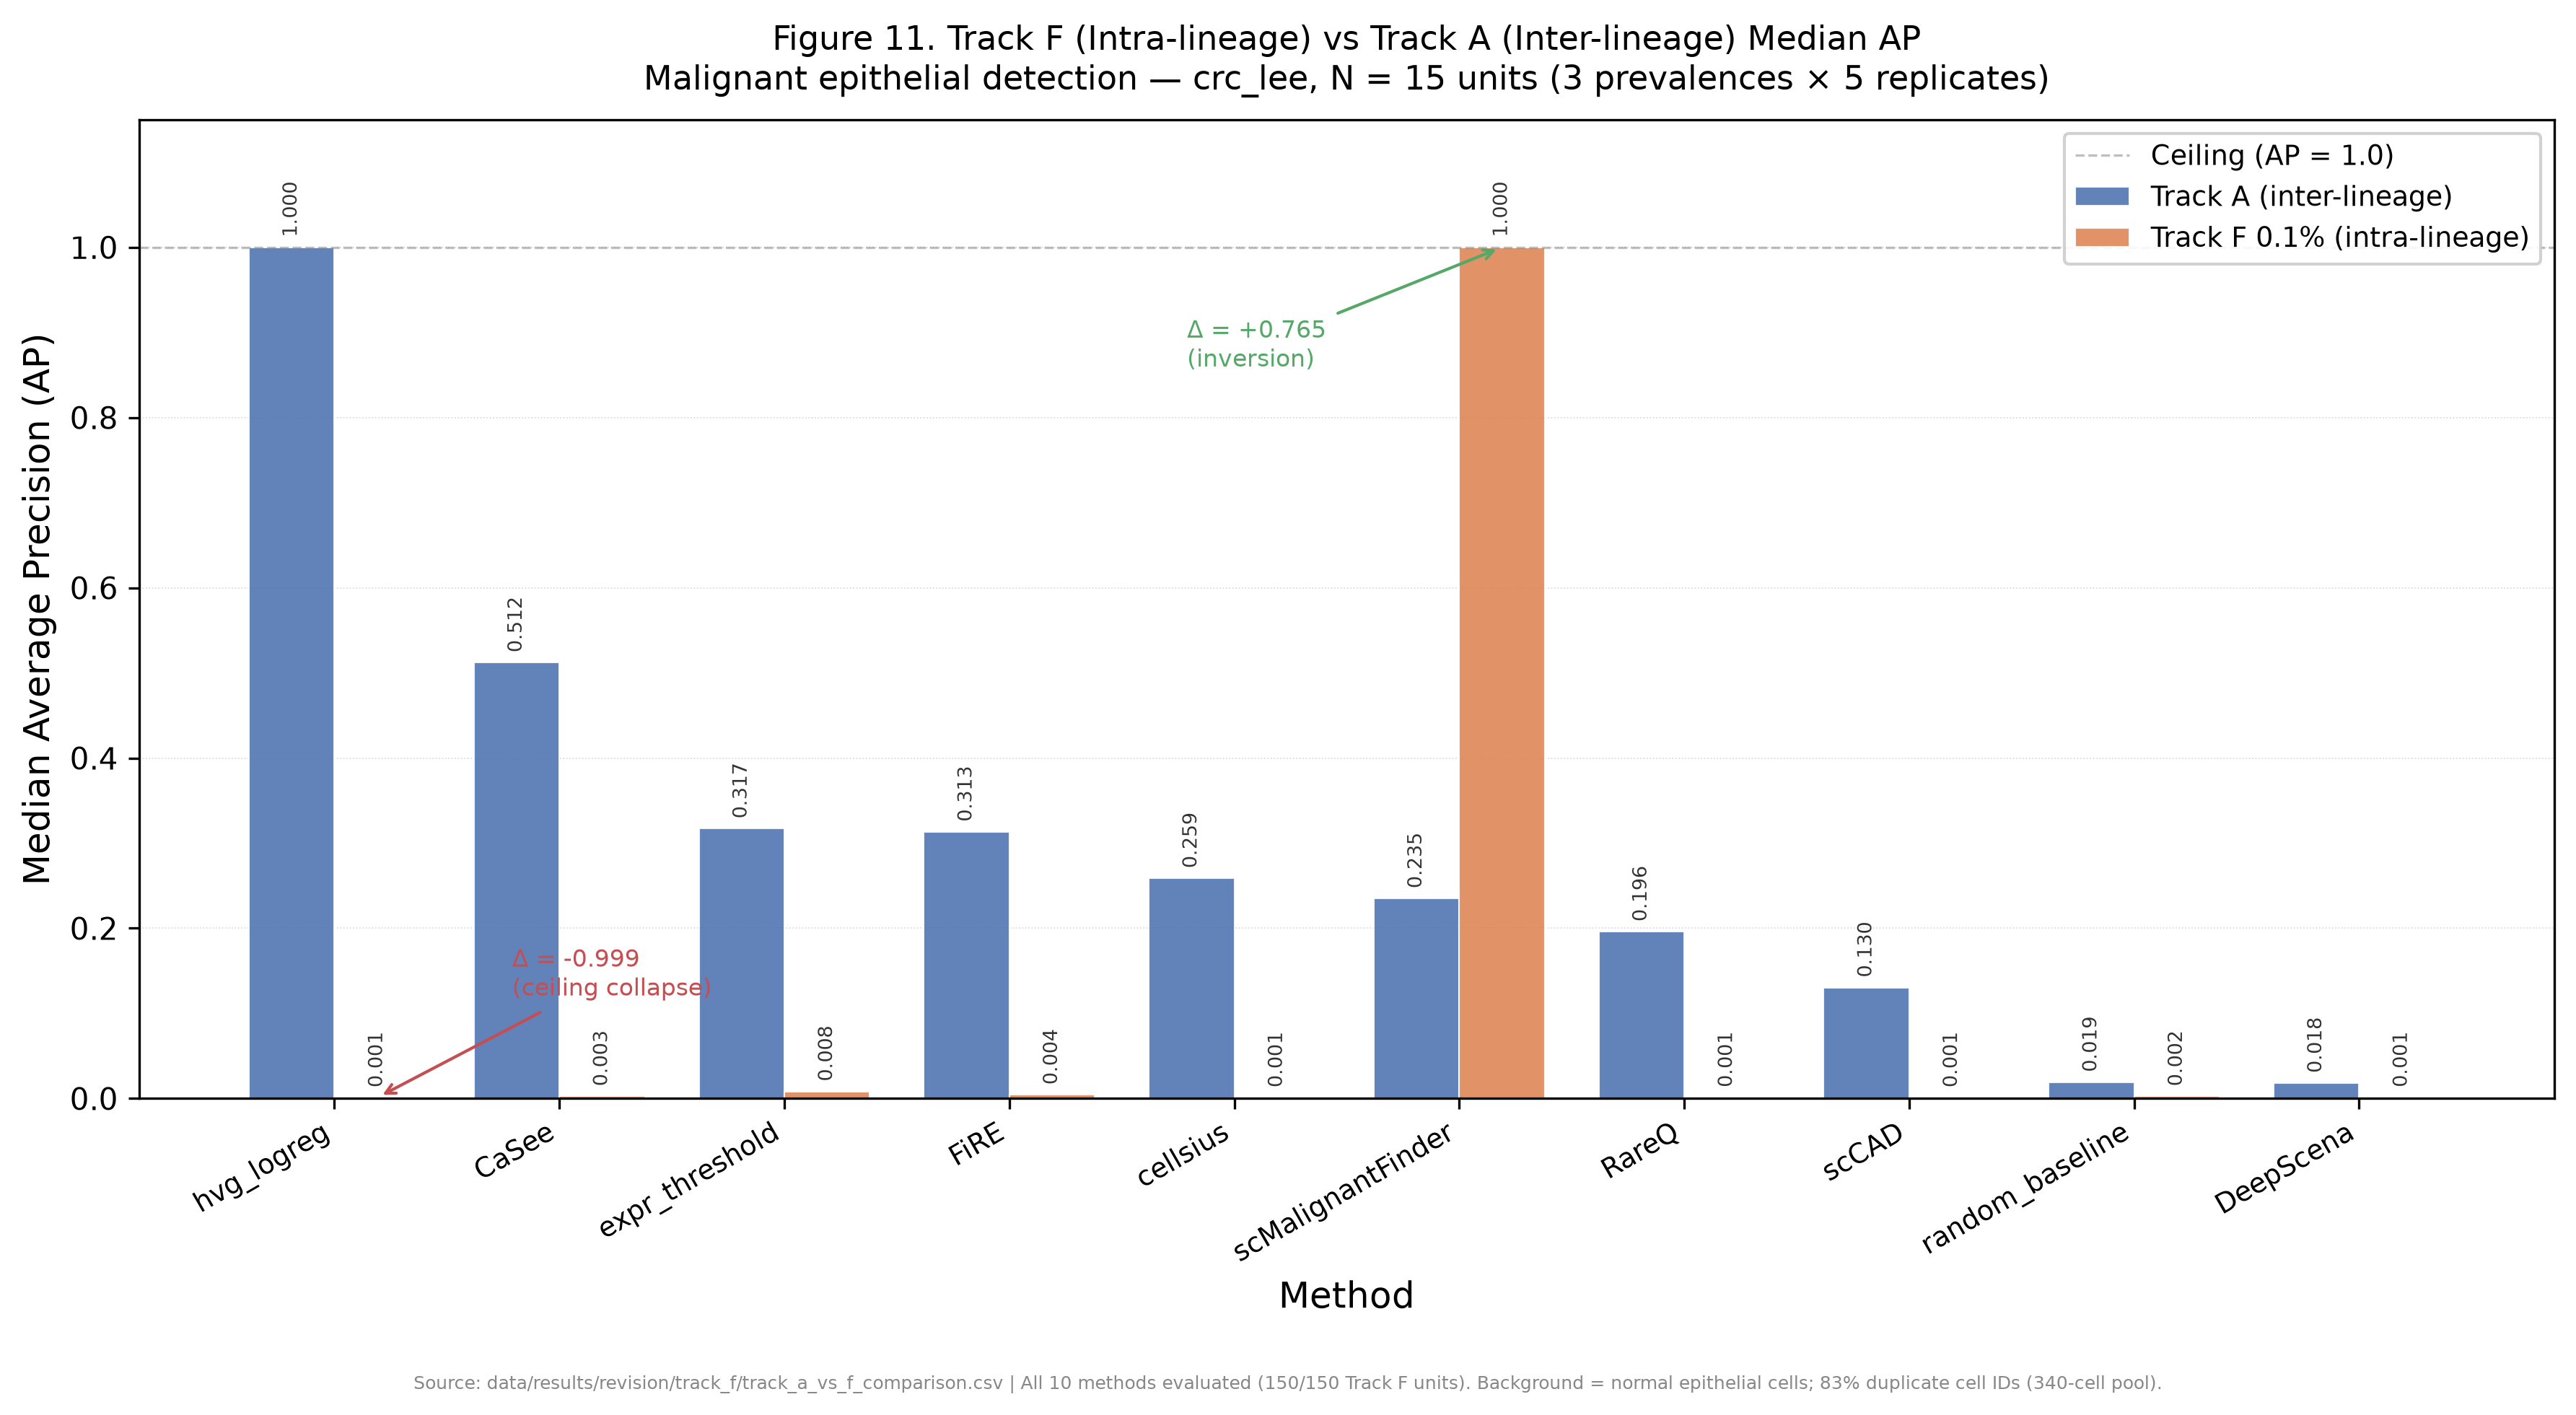
\includegraphics{images/Fig11_Track_F_vs_Track_A.png}
\caption{\DIFaddFL{Figure 11. Track F (intra-lineage) vs Track A (inter-lineage)
median AP per method. hvg\_logreg ceiling collapses from 1.000 to 0.001;
scMalignantFinder inverts (0.235 to 1.000).}}
\end{figure}

\begin{center}\DIFaddFL{\rule{0.5\linewidth}{0.5pt}}\end{center}

\subsection{\DIFaddFL{Dataset-Level Winners}}\label{dataset-level-winners}

\begin{longtable}[]{@{}lll@{}}
\DIFaddendFL \toprule\DIFaddbeginFL \noalign{}
\DIFaddendFL Dataset & \DIFdelbeginFL \DIFdelFL{Best overall }%DIFDELCMD < & %%%
\DIFdelFL{AP }%DIFDELCMD < & %%%
\DIFdelFL{Best non ceiling }%DIFDELCMD < & %%%
\DIFdelFL{AP }\DIFdelendFL \DIFaddbeginFL \DIFaddFL{Best non-ceiling }& \DIFaddFL{AP }\DIFaddendFL \\
\midrule\DIFdelbeginFL \texttt{\DIFdelFL{bcc\_yost}}        %DIFAUXCMD
%DIFDELCMD < & %%%
\texttt{\DIFdelFL{hvg\_logreg}}     %DIFAUXCMD
%DIFDELCMD < & %%%
\DIFdelFL{1.0000 }\DIFdelendFL \DIFaddbeginFL \noalign{}
\endhead
\bottomrule\noalign{}
\endlastfoot
\DIFaddFL{bcc\_yost }\DIFaddendFL & \DIFdelbeginFL \texttt{\DIFdelFL{CaSee}}             %DIFAUXCMD
\DIFdelendFL \DIFaddbeginFL \DIFaddFL{CaSee }\DIFaddendFL & 0.6079 \\
\DIFdelbeginFL \texttt{\DIFdelFL{hnscc\_puram}}     %DIFAUXCMD
%DIFDELCMD < & %%%
\texttt{\DIFdelFL{hvg\_logreg}}     %DIFAUXCMD
%DIFDELCMD < & %%%
\DIFdelFL{1.0000 }\DIFdelendFL \DIFaddbeginFL \DIFaddFL{hnscc\_puram }\DIFaddendFL & \DIFdelbeginFL \texttt{\DIFdelFL{expr\_threshold}}   %DIFAUXCMD
\DIFdelendFL \DIFaddbeginFL \DIFaddFL{expr\_threshold }\DIFaddendFL & 0.7872 \\
\DIFdelbeginFL \texttt{\DIFdelFL{pdac\_peng}}       %DIFAUXCMD
%DIFDELCMD < & %%%
\texttt{\DIFdelFL{hvg\_logreg}}     %DIFAUXCMD
%DIFDELCMD < & %%%
\DIFdelFL{1.0000 }\DIFdelendFL \DIFaddbeginFL \DIFaddFL{pdac\_peng }\DIFaddendFL & \DIFdelbeginFL \texttt{\DIFdelFL{CaSee}}             %DIFAUXCMD
\DIFdelendFL \DIFaddbeginFL \DIFaddFL{CaSee }\DIFaddendFL & 0.4488 \\
\DIFdelbeginFL \texttt{\DIFdelFL{rcc\_multi}}       %DIFAUXCMD
%DIFDELCMD < & %%%
\texttt{\DIFdelFL{hvg\_logreg}}     %DIFAUXCMD
%DIFDELCMD < & %%%
\DIFdelFL{1.0000 }\DIFdelendFL \DIFaddbeginFL \DIFaddFL{rcc\_multi }\DIFaddendFL & \DIFdelbeginFL \texttt{\DIFdelFL{cellsius}}          %DIFAUXCMD
\DIFdelendFL \DIFaddbeginFL \DIFaddFL{cellsius }\DIFaddendFL & 0.1931 \\
\DIFdelbeginFL \texttt{\DIFdelFL{crc\_lee}}         %DIFAUXCMD
%DIFDELCMD < & %%%
\texttt{\DIFdelFL{hvg\_logreg}}     %DIFAUXCMD
%DIFDELCMD < & %%%
\DIFdelFL{0.9998 }\DIFdelendFL \DIFaddbeginFL \DIFaddFL{crc\_lee }\DIFaddendFL & \DIFdelbeginFL \texttt{\DIFdelFL{scMalignantFinder}} %DIFAUXCMD
\DIFdelendFL \DIFaddbeginFL \DIFaddFL{scMalignantFinder }\DIFaddendFL & 0.8373 \\
\DIFdelbeginFL \texttt{\DIFdelFL{luad\_laughney}}   %DIFAUXCMD
%DIFDELCMD < & %%%
\texttt{\DIFdelFL{hvg\_logreg}}     %DIFAUXCMD
%DIFDELCMD < & %%%
\DIFdelFL{0.9983 }\DIFdelendFL \DIFaddbeginFL \DIFaddFL{luad\_laughney }\DIFaddendFL & \DIFdelbeginFL \texttt{\DIFdelFL{CaSee}}             %DIFAUXCMD
\DIFdelendFL \DIFaddbeginFL \DIFaddFL{CaSee }\DIFaddendFL & 0.5378 \\
\DIFdelbeginFL \texttt{\DIFdelFL{hcc\_wei}}         %DIFAUXCMD
%DIFDELCMD < & %%%
\texttt{\DIFdelFL{hvg\_logreg}}     %DIFAUXCMD
%DIFDELCMD < & %%%
\DIFdelFL{0.9948 }\DIFdelendFL \DIFaddbeginFL \DIFaddFL{hcc\_wei }\DIFaddendFL & \DIFdelbeginFL \texttt{\DIFdelFL{CaSee}}             %DIFAUXCMD
\DIFdelendFL \DIFaddbeginFL \DIFaddFL{CaSee }\DIFaddendFL & 0.4908 \\
\DIFdelbeginFL \texttt{\DIFdelFL{ov\_izar\_tirosh}} %DIFAUXCMD
%DIFDELCMD < & %%%
\texttt{\DIFdelFL{expr\_threshold}} %DIFAUXCMD
%DIFDELCMD < & %%%
\DIFdelFL{0.5717 }\DIFdelendFL \DIFaddbeginFL \DIFaddFL{ov\_izar\_tirosh }\DIFaddendFL & \DIFdelbeginFL \texttt{\DIFdelFL{expr\_threshold}}   %DIFAUXCMD
\DIFdelendFL \DIFaddbeginFL \DIFaddFL{expr\_threshold }\DIFaddendFL & 0.5717 \\
\DIFdelbeginFL %DIFDELCMD < \bottomrule
%DIFDELCMD < \end{tabular}
%DIFDELCMD < %%%
\DIFdelendFL \DIFaddbeginFL \end{longtable}
\DIFaddendFL 

\DIFdelbeginFL %DIFDELCMD < \end{table}
%DIFDELCMD < %%%
\DIFdelend \DIFaddbegin \begin{center}\DIFadd{\rule{0.5\linewidth}{0.5pt}}\end{center}
\DIFaddend 

\DIFdelbegin %DIFDELCMD < \subsection{%%%
\DIFdel{Statistical significance and rank uncertainty}%DIFDELCMD < \MBLOCKRIGHTBRACE
%DIFDELCMD < %%%
\DIFdelend \DIFaddbegin \subsection{\DIFadd{Limitations}}\label{limitations}
\DIFaddend 

\DIFdelbegin \DIFdel{The overall rank tests have been conducted on the 140 common unit Track A subset. These tests showed significant differences across methods: Friedman $\chi^2 = 695.05$, $p < 0.001$}\DIFdelend \DIFaddbegin \begin{enumerate}
\def\labelenumi{\arabic{enumi}.}
\tightlist
\item
  \textbf{\DIFadd{CNV evidence, circularity check, and validation.}} \DIFadd{Version 1
  uses infercnvpy (v0.6.1) as the sole copy-number inference arm. To
  assess whether the CNV arm circularly inflates the method ranking, we
  re-derived HC labels using only tissue-of-origin, AUCell signature
  scores, and kNN neighbourhood purity --- dropping the CNV criterion
  entirely --- and recomputed median AP for each method. Removing CNV
  from the label criteria collapses median AP to the chance floor
  (0.009--0.010) for every method including the supervised ceiling,
  indicating that CNV is the primary discriminative signal in the HC
  label set. The rank ordering under CNV-free labels correlates with the
  published ranking (Spearman ρ = 0.648, p = 0.043}\DIFaddend ;
  \DIFdelbegin \DIFdel{Iman-Davenport $F = 171.01$, $p < 0.001$ \mbox{%DIFAUXCMD
\cite{davis2006relationship,saito2015precision}}\hskip0pt%DIFAUXCMD
. The results of the pairwise Wilcoxon tests relative to FiRE (Table 6)
suggest that FiRE has significantly better performance than random baseline}\DIFdelend \DIFaddbegin \texttt{\DIFadd{data/results/revision/circularity\_ranking.csv}}\DIFadd{), but this
  correlation is computed over near-tied chance-level values, so it
  should be interpreted cautiously: the rank order is broadly preserved,
  but the absolute performance differences vanish without CNV. We
  therefore frame CNV as the dominant but not sole label component ---
  tissue-of-origin and signature scores contribute to the HC set but CNV
  drives the discriminability. We also validated inferred CNV burden
  (mean absolute deviation from the diploid baseline) against published
  source malignancy annotations across 9 datasets (57,811 cells; 5}\DIFaddend ,\DIFdelbegin \DIFdel{DeepScena, scCAD}\DIFdelend \DIFaddbegin \DIFadd{010
  positive; 52}\DIFaddend ,\DIFdelbegin \DIFdel{RareQ and cellsius ($p < 0.05$ after Benjamini-Hochberg FDR correction).
  There are no significant differences between scMalignantFinder and exprthreshold methods when compared to FiRE. In our exploratory comparison, CaSee is better than FiRE ($\Delta$mean AP }\DIFdelend \DIFaddbegin \DIFadd{801 background;
  }\texttt{\DIFadd{data/results/revision/cnv\_concordance.csv}}\DIFadd{). CNV burden
  discriminated source-annotated malignant from non-malignant cells with
  overall AUROC }\DIFaddend = \DIFdelbegin \DIFdel{$-0.140$}\DIFdelend \DIFaddbegin \DIFadd{0.782 and MCC = 0.361. Per-dataset AUROC ranged from
  0.747 (hcc\_wei) to 0.960 (luad\_laughney), with five datasets
  exceeding 0.86 (luad\_laughney 0.960, pdac\_peng 0.934, crc\_lee
  0.892, hnscc\_puram 0.906, ov\_izar\_tirosh 0.868). An earlier version
  of this analysis reported hnscc\_puram at AUROC = 0.500 because its
  }\texttt{\DIFadd{cell\_type}} \DIFadd{labels (e.g.~}\texttt{\DIFadd{"0.0"}}\DIFaddend ,
  \DIFdelbegin \DIFdel{BH FDR }\DIFdelend \DIFaddbegin \texttt{\DIFadd{"Fibroblast"}}\DIFadd{, }\texttt{\DIFadd{"T\ cell"}}\DIFadd{) did not match infercnvpy's
  default reference categories (}\texttt{\DIFadd{T\ cells}}\DIFadd{, }\texttt{\DIFadd{B\ cells}}\DIFadd{,
  }\texttt{\DIFadd{Myeloids}}\DIFadd{, \ldots) and CNV scores were zero; we corrected the
  reference categories to include the singular label forms present in
  this dataset and regenerated its CNV, yielding AUROC }\DIFaddend = \DIFdelbegin \DIFdel{$6.1 \times 10^{-8}$; Cliff’s $\delta = -0.245$) ; this is reported under the exploratoryversus published category, not under the primary ranked method category \mbox{%DIFAUXCMD
\cite{sh2022casee}}\hskip0pt%DIFAUXCMD
.
}\DIFdelend \DIFaddbegin \DIFadd{0.906 (MCC =
  0.763). CNV is therefore used as one of three independent HC-label
  components, not as a standalone ground truth. Cross-validation with
  CopyKAT, Numbat, or SCEVAN would further strengthen CNV evidence but
  was not feasible at this scale.
}\item
  \textbf{\DIFadd{Imperfect ground truth.}} \DIFadd{High-confidence labels (P\_HC/B\_HC)
  rely on consensus across four evidence arms. False positives in source
  annotation or CNV calls can propagate. The tier-assignment system
  mitigates this by using only P\_HC vs B\_HC for primary AP
  computation.
}\item
  \textbf{\DIFadd{Fallback and degenerate rates.}} \DIFadd{Across all methods, 249 units
  produced fallback scores and 377 units produced degenerate outputs.
  These rates are high and reflect current engineering stability
  limitations of method wrappers rather than algorithmic quality.
}\item
  \textbf{\DIFadd{Dataset diversity.}} \DIFadd{The 10 datasets span 8 solid-tumour types
  and 2 blood malignancies but are dominated by 10x Chromium (8/10).
  SMART-seq2 is represented in only 2 datasets. No spatial
  transcriptomics or multi-omics data are included.
}\item
  \textbf{\DIFadd{Track D size.}} \DIFadd{Natural prevalence evaluation (Track D)
  contains only 30 units from 2 datasets, limiting statistical power for
  this track.
}\item
  \textbf{\DIFadd{No held-out datasets.}} \DIFadd{All datasets are public. Method
  developers can tune against the leaderboard, though REACH's
  multi-track design with null controls and label-noise tracks makes
  simple overfitting harder.
}\item
  \textbf{\DIFadd{Single contributor.}} \DIFadd{The benchmark was developed by a single
  author. Independent verification by additional researchers would
  strengthen reproducibility claims.
}\item
  \textbf{\DIFadd{Cancer-type scope.}} \DIFadd{Several therapeutically important cancer
  types (glioblastoma, prostate adenocarcinoma, gastric cancer) are not
  represented.
}\item
  \textbf{\DIFadd{Label-threshold sensitivity.}} \DIFadd{To test whether the qualitative
  method ordering depends on the AUCell score threshold and kNN
  neighbourhood-purity cutoff, we varied both across nine combinations
  (AUCell 0.10/0.15/0.20 × kNN 0.40/0.50/0.60) while holding CNV scores
  fixed, and recomputed rankings. On the five datasets yielding a valid
  Spearman ρ, the high-confidence label sets were insensitive to these
  threshold variations --- the same cells were selected at every setting
  --- so the resulting method rankings are identical within each dataset
  (ρ per dataset: luad\_laughney 0.685, pdac\_peng 0.758, bcc\_yost
  0.818, hcc\_wei 0.879, crc\_lee 0.939). The cross-dataset ρ range
  }{[}\DIFadd{0.685, 0.939}{]} \DIFadd{therefore reflects dataset-level variation in label
  separability, not threshold sensitivity. Two datasets
  (ov\_izar\_tirosh, rcc\_multi) could not form a high-confidence
  background at any setting (n\_B\_HC = 0) and are excluded. The
  label-construction pipeline is thus stable to the tested threshold
  parameters, though this analysis does not demonstrate ranking
  robustness to threshold changes that would actually alter the label
  set (}\texttt{\DIFadd{data/results/revision/threshold\_sensitivity.csv}}\DIFadd{).
}\item
  \textbf{\DIFadd{TME overlap and the false-positive scope choice.}} \DIFadd{Because
  REACH measures detection against a heterogeneous TME background,
  methods trained or implicitly calibrated on the malignant-vs-TME
  contrast may flag TME subpopulations whose expression partially
  overlaps malignant signatures (e.g.~activated macrophages,
  plasmablasts, cycling fibroblasts) as false positives. This is a
  deliberate scope choice: REACH models the realistic low-prevalence
  screening scenario in which TME is the background and tolerance to
  such false positives is modulated by precision@k. Track C confirms
  that, on pure all-negative null units, every unsupervised method keeps
  its mean FPR near 3\%
  (}\texttt{\DIFadd{data/results/revision/sens2\_sens3\_extract.txt}}\DIFadd{), so
  elevated FPR on mixed-TME units reflects biological overlap, not
  metric pathology. The new intra-lineage Track F (R3-4/R3-5) begins to
  disentangle behaviour on pure-epithelial versus mixed-TME backgrounds.
}\end{enumerate}
\DIFaddend 

\DIFdelbegin %DIFDELCMD < \begin{table}[H]
%DIFDELCMD < \centering
%DIFDELCMD < %%%
%DIFDELCMD < \caption{%
{%DIFAUXCMD
\DIFdelFL{Selected pairwise comparisons on Track A AP from
}\texttt{\DIFdelFL{pairwise\_tests.csv}}%DIFAUXCMD
\DIFdelFL{. Positive $\Delta$ means }\texttt{\DIFdelFL{FiRE}} %DIFAUXCMD
\DIFdelFL{has
higher mean AP than the comparator; negative $\Delta$ means the
comparator has higher mean AP.}}
%DIFAUXCMD
%DIFDELCMD < \label{tab:pairwise}
%DIFDELCMD < \small
%DIFDELCMD < \begin{tabular}{lrrrr}
%DIFDELCMD < %%%
\DIFdelendFL \DIFaddbeginFL \begin{center}\DIFaddFL{\rule{0.5\linewidth}{0.5pt}}\end{center}

\subsection{\DIFaddFL{Comparison to Related
Benchmarks}}\label{comparison-to-related-benchmarks}

\begin{longtable}[]{@{}
  >{\raggedright\arraybackslash}p{(\columnwidth - 6\tabcolsep) * \real{0.1304}}
  >{\raggedright\arraybackslash}p{(\columnwidth - 6\tabcolsep) * \real{0.1739}}
  >{\raggedright\arraybackslash}p{(\columnwidth - 6\tabcolsep) * \real{0.3043}}
  >{\raggedright\arraybackslash}p{(\columnwidth - 6\tabcolsep) * \real{0.3913}}@{}}
\DIFaddendFL \toprule\DIFdelbeginFL \DIFdelFL{Comparator }%DIFDELCMD < & %%%
\DIFdelFL{$\Delta$ mean AP }\DIFdelendFL \DIFaddbeginFL \noalign{}
\begin{minipage}[b]{\linewidth}\raggedright
\DIFaddFL{Feature
}\end{minipage} \DIFaddendFL & \DIFdelbeginFL \DIFdelFL{Wilcoxon $p$ }\DIFdelendFL \DIFaddbeginFL \begin{minipage}[b]{\linewidth}\raggedright
\DIFaddFL{REACH v1.2
}\end{minipage} \DIFaddendFL & \DIFdelbeginFL \DIFdelFL{BH FDR }\DIFdelendFL \DIFaddbeginFL \begin{minipage}[b]{\linewidth}\raggedright
\DIFaddFL{scIB (Luecken 2022)
}\end{minipage} \DIFaddendFL & \DIFdelbeginFL \DIFdelFL{Cliff's $\delta$ }\DIFdelendFL \DIFaddbeginFL \begin{minipage}[b]{\linewidth}\raggedright
\DIFaddFL{OpenProblems (Lance 2024)
}\end{minipage} \DIFaddendFL \\
\midrule\DIFdelbeginFL \texttt{\DIFdelFL{DeepScena}}        %DIFAUXCMD
%DIFDELCMD < &  %%%
\DIFdelFL{0.3320 }\DIFdelendFL \DIFaddbeginFL \noalign{}
\endhead
\bottomrule\noalign{}
\endlastfoot
\DIFaddFL{Task }\DIFaddendFL & \DIFdelbeginFL \DIFdelFL{$1.10\!\times\!10^{-24}$ }\DIFdelendFL \DIFaddbeginFL \DIFaddFL{Rare malignant cell detection }\DIFaddendFL & \DIFdelbeginFL \DIFdelFL{$1.66\!\times\!10^{-23}$ }\DIFdelendFL \DIFaddbeginFL \DIFaddFL{Batch correction, clustering,
integration }\DIFaddendFL & \DIFdelbeginFL \DIFdelFL{0.7539 }\DIFdelendFL \DIFaddbeginFL \DIFaddFL{Multi-task (denoising, DE, etc.) }\DIFaddendFL \\
\DIFdelbeginFL \texttt{\DIFdelFL{random\_baseline}} %DIFAUXCMD
%DIFDELCMD < &  %%%
\DIFdelFL{0.3226 }\DIFdelendFL \DIFaddbeginFL \DIFaddFL{Tracks }\DIFaddendFL & \DIFdelbeginFL \DIFdelFL{$2.52\!\times\!10^{-22}$ }\DIFdelendFL \DIFaddbeginFL \DIFaddFL{6 (spike-in, synthetic, null, natural, noise, intra-lineage) }\DIFaddendFL &
\DIFdelbeginFL \DIFdelFL{$8.11\!\times\!10^{-22}$ }\DIFdelendFL \DIFaddbeginFL \DIFaddFL{Multi-metric per task }\DIFaddendFL & \DIFdelbeginFL \DIFdelFL{0.7271 }\DIFdelendFL \DIFaddbeginFL \DIFaddFL{Per-task metrics }\DIFaddendFL \\
\DIFdelbeginFL \texttt{\DIFdelFL{CaSee}}            %DIFAUXCMD
%DIFDELCMD < & %%%
\DIFdelFL{-0.1395 }\DIFdelendFL \DIFaddbeginFL \DIFaddFL{Labels }\DIFaddendFL & \DIFdelbeginFL \DIFdelFL{$3.96\!\times\!10^{-8}$  }\DIFdelendFL \DIFaddbeginFL \DIFaddFL{Multi-arm confidence tiers (P\_HC-B\_LC) }\DIFaddendFL & \DIFdelbeginFL \DIFdelFL{$6.14\!\times\!10^{-8}$  }\DIFdelendFL \DIFaddbeginFL \DIFaddFL{Canonical cell-type
labels }\DIFaddendFL & \DIFdelbeginFL \DIFdelFL{-0.2451 }\DIFdelendFL \DIFaddbeginFL \DIFaddFL{Truth from data generators }\DIFaddendFL \\
\DIFdelbeginFL \texttt{\DIFdelFL{scCAD}}            %DIFAUXCMD
%DIFDELCMD < &  %%%
\DIFdelFL{0.1350 }\DIFdelendFL \DIFaddbeginFL \DIFaddFL{Null controls }\DIFaddendFL & \DIFdelbeginFL \DIFdelFL{$1.56\!\times\!10^{-4}$  }\DIFdelendFL \DIFaddbeginFL \DIFaddFL{Yes (Track C) }\DIFaddendFL & \DIFdelbeginFL \DIFdelFL{$2.34\!\times\!10^{-4}$  }\DIFdelendFL \DIFaddbeginFL \DIFaddFL{Not standard }\DIFaddendFL & \DIFdelbeginFL \DIFdelFL{0.2886 }\DIFdelendFL \DIFaddbeginFL \DIFaddFL{Not standard }\DIFaddendFL \\
\DIFdelbeginFL \texttt{\DIFdelFL{RareQ}}            %DIFAUXCMD
%DIFDELCMD < &  %%%
\DIFdelFL{0.1161 }\DIFdelendFL \DIFaddbeginFL \DIFaddFL{Label noise }\DIFaddendFL & \DIFdelbeginFL \DIFdelFL{$1.77\!\times\!10^{-3}$  }\DIFdelendFL \DIFaddbeginFL \DIFaddFL{Yes (Track E, supervised only) }\DIFaddendFL & \DIFdelbeginFL \DIFdelFL{$2.49\!\times\!10^{-3}$  }\DIFdelendFL \DIFaddbeginFL \DIFaddFL{Not included }\DIFaddendFL & \DIFdelbeginFL \DIFdelFL{0.2457 }\DIFdelendFL \DIFaddbeginFL \DIFaddFL{Not
included }\DIFaddendFL \\
\DIFdelbeginFL \texttt{\DIFdelFL{cellsius}}         %DIFAUXCMD
%DIFDELCMD < &  %%%
\DIFdelFL{0.0978 }\DIFdelendFL \DIFaddbeginFL \DIFaddFL{Supervised ceiling }\DIFaddendFL & \DIFdelbeginFL \DIFdelFL{$3.06\!\times\!10^{-3}$  }\DIFdelendFL \DIFaddbeginFL \DIFaddFL{Yes (hvg\_logreg) }\DIFaddendFL & \DIFdelbeginFL \DIFdelFL{$4.04\!\times\!10^{-3}$  }\DIFdelendFL \DIFaddbeginFL \DIFaddFL{Not standard }\DIFaddendFL & \DIFdelbeginFL \DIFdelFL{0.1930 }\DIFdelendFL \DIFaddbeginFL \DIFaddFL{Not standard }\DIFaddendFL \\
\DIFdelbeginFL \texttt{\DIFdelFL{scMalignantFinder}}%DIFAUXCMD
%DIFDELCMD < &  %%%
\DIFdelFL{0.0453 }\DIFdelendFL \DIFaddbeginFL \DIFaddFL{Fallback handling }\DIFaddendFL & \DIFdelbeginFL \DIFdelFL{0.812                    }\DIFdelendFL \DIFaddbeginFL \DIFaddFL{Filtered from primary AP }\DIFaddendFL & \DIFdelbeginFL \DIFdelFL{0.831                    }\DIFdelendFL \DIFaddbeginFL \DIFaddFL{Not standardised }\DIFaddendFL &
\DIFdelbeginFL \DIFdelFL{0.1206 }\DIFdelendFL \DIFaddbeginFL \DIFaddFL{Varies }\DIFaddendFL \\
\DIFdelbeginFL \texttt{\DIFdelFL{expr\_threshold}}  %DIFAUXCMD
%DIFDELCMD < &  %%%
\DIFdelFL{0.0304 }\DIFdelendFL \DIFaddbeginFL \DIFaddFL{Containerisation }\DIFaddendFL & \DIFdelbeginFL \DIFdelFL{0.836                    }\DIFdelendFL \DIFaddbeginFL \DIFaddFL{Docker + GHCR }\DIFaddendFL & \DIFdelbeginFL \DIFdelFL{0.836                    }\DIFdelendFL \DIFaddbeginFL \DIFaddFL{Docker }\DIFaddendFL & \DIFdelbeginFL \DIFdelFL{0.0816 }\DIFdelendFL \DIFaddbeginFL \DIFaddFL{Docker + Nextflow }\DIFaddendFL \\
\DIFdelbeginFL %DIFDELCMD < \bottomrule
%DIFDELCMD < \end{tabular}
%DIFDELCMD < \end{table}
%DIFDELCMD < %%%
\DIFdelend \DIFaddbegin \end{longtable}
\DIFaddend 

\DIFdelbegin \DIFdel{The bootstrap intervals for ranks are stable, whereas the hvglogreg and CaSee methods are ranked 1 and 2 respectively for every resample of 2, 000. On the other hand, FiRE is observed to have a median rank of 3 (with a 95\% bootstrap rank interval of }%DIFDELCMD < [%%%
\DIFdel{3, 4}%DIFDELCMD < ]%%%
\DIFdel{). Expr threshold
  , scMalignantFinder, cellsius, RareQ, and scCAD fall into an overlapping middle band (Fig.~\ref{fig:fig4}(a)). The mean within-unit rank for each method, shown in Fig.~\ref{fig:fig4}(b) , separates the strongest methods from the overlapping middle group and is consistent with the bootstrap rank intervals \mbox{%DIFAUXCMD
\cite{gorodkin2004comparing}}\hskip0pt%DIFAUXCMD
.
}\DIFdelend \DIFaddbegin \begin{center}\DIFadd{\rule{0.5\linewidth}{0.5pt}}\end{center}
\DIFaddend 

\DIFdelbegin \subsection{\DIFdel{Rarity sensitivity and track specific robustness}}
%DIFAUXCMD
\addtocounter{subsection}{-1}%DIFAUXCMD
\DIFdel{Rarity sensitivity was assessed by regressing nAP against $\log_{10}(\pi_u)$, where $\pi_u$ denotes the positive-cell prevalence in each benchmark unit (Fig.~\ref{fig:fig4}(c)). Most methods show positive slopes, indicating that performance improved as rare cells became less sparse.
CellSIUS shows the largest nAP slope ($0.220$}\DIFdelend \DIFaddbegin \subsection{\DIFadd{Data and Code
Availability}}\label{data-and-code-availability}

\begin{itemize}
\tightlist
\item
  \textbf{\DIFadd{Source code:}}
  \DIFadd{https://github.com/jaswanthmoram/reach-rarecell-benchmark
}\item
  \textbf{\DIFadd{Concept DOI:}} \DIFadd{https://doi.org/10.5281/zenodo.19847108
}\item
  \textbf{\DIFadd{Processed datasets (7.3 GB):}}
  \DIFadd{https://doi.org/10.5281/zenodo.19850652
}\item
  \textbf{\DIFadd{Track Units A-C (9.7 GB):}}
  \DIFadd{https://doi.org/10.5281/zenodo.19850972
}\item
  \textbf{\DIFadd{Track Units D-E (2.2 GB):}}
  \DIFadd{https://doi.org/10.5281/zenodo.19851287
}\item
  \textbf{\DIFadd{Complete results (425 MB):}}
  \DIFadd{https://doi.org/10.5281/zenodo.19851710
}\item
  \textbf{\DIFadd{Docker image:}}
  \DIFadd{ghcr.io/jaswanthmoram/reach-rarecell-benchmark:latest
}\item
  \textbf{\DIFadd{License:}} \DIFadd{MIT
}\item
  \textbf{\DIFadd{GEO accessions:}} \DIFadd{GSE103322}\DIFaddend , \DIFdelbegin \DIFdel{$p = 1.78 \times 10^{-20}$)}\DIFdelend \DIFaddbegin \DIFadd{GSE123813}\DIFaddend , \DIFdelbegin \DIFdel{while RareQ, CaSee, scMalignantFinder, scCAD, FiRE, and exprthreshold show similar positive slopes. These nAP slopes are descriptive \mbox{%DIFAUXCMD
\cite{johnson2019survey,altalhan2025imbalanced}}\hskip0pt%DIFAUXCMD
.
}%DIFDELCMD < 

%DIFDELCMD < %%%
\DIFdel{There is a reordering of methods in Track B versus Track A (Spearman rank correlation $\rho = 0.042$}\DIFdelend \DIFaddbegin \DIFadd{GSE149614}\DIFaddend , \DIFdelbegin \DIFdel{$p = 0.907$, so the Track B stands as a stress test versus being incorporated into the primary leaderboard (Fig.~\ref{fig:fig5}(a), left side) \mbox{%DIFAUXCMD
\cite{cao2021benchmark}}\hskip0pt%DIFAUXCMD
. The track E hvg-logreg label noise analysis shows that the loss in mean AP is relative to a Track A mean AP of $0.9088$: hvg-logreg mean AP drops between $0.909$ and $0.534$ under $30\% $ background-to-positive flips, $0.829$ under $30\%$ positive to background flips, $0.481$ under $10\%$ symmetric noise and $0.460$ under $20\%$ symmetric noise.
  On the other hand, the corresponding robustness indices (ranging from 0 to 1) for these analyses are $0.588$}\DIFdelend \DIFaddbegin \DIFadd{GSE123902}\DIFaddend ,
  \DIFdelbegin \DIFdel{$0.912$}\DIFdelend \DIFaddbegin \DIFadd{GSE202051}\DIFaddend , \DIFdelbegin \DIFdel{$0.529$}\DIFdelend \DIFaddbegin \DIFadd{GSE132465}\DIFaddend , \DIFdelbegin \DIFdel{$0.507$ respectively (Fig.~\ref{fig:fig5} (a), right side) \mbox{%DIFAUXCMD
\cite{mahalanabis2022evaluation}}\hskip0pt%DIFAUXCMD
.
}\DIFdelend \DIFaddbegin \DIFadd{GSE159115, GSE146026, GSE161801, GSE109761
}\end{itemize}
\DIFaddend 

\DIFdelbegin \subsection{\DIFdel{Null behavior and calibration}}
%DIFAUXCMD
\addtocounter{subsection}{-1}%DIFAUXCMD
\DIFdelend \DIFaddbegin \DIFadd{Git alone is sufficient for toy workflows and public snapshot
reproduction. Full processed-data, track-unit, prediction, and
complete-result reruns require restoring the external Zenodo archives
listed above.
}\DIFaddend 

\DIFdelbegin \DIFdel{Track C evaluates false-positive behavior in background dominated units, where no true rare malignant cells are expected (Fig.~\ref{fig:fig5}(b)) \mbox{%DIFAUXCMD
\cite{torre2018rare}}\hskip0pt%DIFAUXCMD
. For each method, REACH measures the fraction of top
  ranked cells that are incorrectly selected as positives under these null-control conditions.
Most unsupervised, exploratory, and naive scoring methods show an average top k false positive rate of approximately 3\% : CaSee = 0.0301, DeepScena = 0.0306, FiRE = 0.0315, RareQ = 0.0293,
  CellSIUS = 0.0295, expr-threshold = 0.0310, scCAD = 0.0301, scMalignantFinder = 0.0315, and random baseline = 0.0309. In contrast, the supervised hvg-logreg ceiling shows a much higher Track C false positive rate of 0.788. This behavior is expected because hvg-logreg is an in-sample supervised ceiling, not a deployable unsupervised detector. Calibration has been assessed only for methods that produced probability-like scores \mbox{%DIFAUXCMD
\cite{christensen2023evaluation,abdelaal2019comparison}}\hskip0pt%DIFAUXCMD
. }\DIFdelend \DIFaddbegin \begin{center}\DIFadd{\rule{0.5\linewidth}{0.5pt}}\end{center}
\DIFaddend 

\DIFdelbegin \subsection{\DIFdel{Runtime, scalability, and failure modes}}
%DIFAUXCMD
\addtocounter{subsection}{-1}%DIFAUXCMD
\DIFdelend \DIFaddbegin \subsection{\DIFadd{Reproducibility}}\label{reproducibility}
\DIFaddend 

\DIFdelbegin \DIFdel{Runtime varies by approximately two orders of magnitude across methods (Fig.~\ref{fig:runtime}). Track A Mean Execution Times (MET) for the corresponding tools range from 3.3 seconds (hvg-logistic regression) to 7.6 seconds (scMalignantFinder)to 357.5 seconds (CaSee)
  ; FiRE MET of 118.1 seconds, scCAD MET of 123.4 seconds,RareQ MET of 78.2 seconds,
  DeepScena MET of 80.6 seconds,
  cellsius MET of 39.8 seconds \mbox{%DIFAUXCMD
\cite{brendel2022application,wang2022comparison}}\hskip0pt%DIFAUXCMD
. Runtime also needs to be put into context with fallback and /or degenerate output behavior. Runtime should therefore be interpreted together with fallback and degenerate-output rates, because a fast method is not necessarily reliable if it frequently returns constant scores or fails on many benchmark units \mbox{%DIFAUXCMD
\cite{everingham2010pascal,tran2020benchmark}}\hskip0pt%DIFAUXCMD
.
}\DIFdelend \DIFaddbegin \subsubsection{\DIFadd{Snapshot Reproduction (Git-only, no external
data)}}\label{snapshot-reproduction-git-only-no-external-data}
\DIFaddend 

\DIFdelbegin %DIFDELCMD < \begin{figure}[H]
%DIFDELCMD < \centering
%DIFDELCMD < 
\includegraphics[
%DIFDELCMD < width=0.95\linewidth,
%DIFDELCMD < height=0.78\textheight,
%DIFDELCMD < keepaspectratio
%DIFDELCMD < ]{figures_final/Fig4_Rank_Uncertainty_Rarity.pdf}
%DIFDELCMD < \caption{%%%
\textbf{\DIFdelFL{Rank uncertainty, critical difference, and rarity sensitivity.}}%DIFAUXCMD
%DIFDELCMD < \\[4pt]
%DIFDELCMD < %%%
\textbf{\DIFdelFL{(a)}} %DIFAUXCMD
\DIFdelFL{Bootstrap rank confidence intervals. Ranks are computed from Track A AP over 2}%DIFDELCMD < {%%%
\DIFdelFL{,}%DIFDELCMD < }%%%
\DIFdelFL{000 unit level bootstrap resamples (}\texttt{\DIFdelFL{rank\_ci.csv}}%DIFAUXCMD
\DIFdelFL{). Lower rank is better. }\textbf{\DIFdelFL{(b)}} %DIFAUXCMD
\DIFdelFL{Critical difference rank view. It shows the mean within unit ranks on the common Track A subset, with the Nemenyi critical difference bar }\DIFdelendFL \DIFaddbeginFL \begin{Shaded}
\begin{Highlighting}[]
\ExtensionTok{rcb}\NormalTok{ smoke{-}test}
\ExtensionTok{python}\NormalTok{ scripts/run\_all.py }\AttributeTok{{-}{-}toy}
\ExtensionTok{python}\NormalTok{ scripts/phase11\_statistics.py }\AttributeTok{{-}{-}from{-}snapshots}
\ExtensionTok{python}\NormalTok{ scripts/reproduce\_from\_snapshots.py}
\ExtensionTok{snakemake} \AttributeTok{{-}n} \AttributeTok{{-}{-}cores}\NormalTok{ 1}
\ExtensionTok{dvc}\NormalTok{ repro }\AttributeTok{{-}{-}dry}
\end{Highlighting}
\end{Shaded}

\DIFaddFL{See }\texttt{\DIFaddFL{docs/reproducibility\_receipt.md}} \DIFaddFL{for the verified execution
record, environment details, and expected outputs.
}

\subsubsection{\DIFaddFL{Revision compute
environment}}\label{revision-compute-environment}

\DIFaddFL{The sensitivity, CNV-validation, Track F, and concordance analyses in
this revision were executed on a single CPU-only node: AMD EPYC 7B12 }\DIFaddendFL (\DIFdelbeginFL \DIFdelFL{CD$\,\approx\,1.14$, $k=10$, $N=140$}\DIFdelendFL \DIFaddbeginFL \DIFaddFL{16
vCPUs), 62 GiB RAM, Debian GNU/Linux 13 trixie, Python 3.13.5, R 4.5.0,
with scanpy 1.12.1}\DIFaddendFL , \DIFdelbeginFL \DIFdelFL{$\alpha=0.05$}\DIFdelendFL \DIFaddbeginFL \DIFaddFL{scikit-learn 1.9.0, infercnvpy 0.6.1, anndata
0.11.4, torch 2.12.1 (CPU). R packages FiRE, CellSIUS, RareQ, and Seurat
were installed and ran natively. }\textbf{\DIFaddFL{No GPU was available on this
node.}} \DIFaddFL{DeepScena, whose TensorFlow/Torch pipeline requires CUDA, was run
separately on a Google Colab Tesla T4 GPU; its predictions were
transferred back and scored identically to all other methods. Full
environment capture:
}\texttt{\DIFaddFL{data/results/revision/environment\_capture.txt}}\DIFaddFL{. (The original
v1.2.0 preprocessing cited in the Acknowledgements used GCP high-memory
CPU and NVIDIA L4 GPU instances; that remains the record for dataset
pre-processing, while the revision compute above is the record for the
new analyses.}\DIFaddendFL )
\DIFdelbeginFL \DIFdelFL{. }\textbf{\DIFdelFL{(c)}} %DIFAUXCMD
\DIFdelFL{Rarity sensitivity. It depicts AP and normalized AP across Track A prevalence tiers T1--T4. Several methods degrade sharply in ultra rare units, while the supervised ceiling remains near $1$ across tiers.}%DIFDELCMD < \MBLOCKRIGHTBRACE
%DIFDELCMD < %%%
\DIFdelendFL 

\DIFdelbeginFL %DIFDELCMD < \label{fig:fig4}
%DIFDELCMD < \end{figure}
%DIFDELCMD < %%%
\DIFdelend \DIFaddbegin \begin{center}\DIFadd{\rule{0.5\linewidth}{0.5pt}}\end{center}
\DIFaddend 

\DIFdelbegin %DIFDELCMD < \begin{figure}[H]
%DIFDELCMD < \centering
%DIFDELCMD < 
\includegraphics[
%DIFDELCMD < width=0.95\linewidth,
%DIFDELCMD < height=0.78\textheight,
%DIFDELCMD < keepaspectratio
%DIFDELCMD < ]{figures_final/Fig5_Track_Sensitivity_Null.pdf}
%DIFDELCMD < \caption{%%%
\textbf{\DIFdelFL{Track sensitivity, robustness, and null behavior.}}%DIFAUXCMD
%DIFDELCMD < \\[4pt]
%DIFDELCMD < %%%
\textbf{\DIFdelFL{(a)}} %DIFAUXCMD
\DIFdelFL{Track sensitivity and supervised label noise diagnostics. Left: Track A vs Track B mean AP per method, with the diagonal showing equal performance. Right: Track E robustness indices for the supervised ceiling under four label perturbations. Track~E is not interpretable for unsupervised methods.}%DIFDELCMD < \\[3pt]
%DIFDELCMD < %%%
\textbf{\DIFdelFL{(b)}} %DIFAUXCMD
\DIFdelFL{Track C null behavior and calibration. Background dominated units assess false positive behavior. ECE is shown only for methods with probability like outputs.}%DIFDELCMD < \MBLOCKRIGHTBRACE
%DIFDELCMD < %%%
\DIFdelendFL \DIFaddbeginFL \subsection{\DIFaddFL{Author}}\label{author}
\DIFaddendFL 

\DIFdelbeginFL %DIFDELCMD < \label{fig:fig5}
%DIFDELCMD < \end{figure}
%DIFDELCMD < %%%
\DIFdelend \DIFaddbegin \textbf{\DIFadd{Moram Venkata Satya Jaswanth}} \DIFadd{Department of Computer Science and
Engineering, SRM University AP, Amaravati, Andhra Pradesh, India Email:
jaswanthmoram@gmail.com ORCID: 0009-0003-2369-1692
}\DIFaddend 

\DIFdelbegin \section{\DIFdel{Discussion}}
%DIFAUXCMD
\addtocounter{section}{-1}%DIFAUXCMD
\DIFdelend \DIFaddbegin \begin{center}\DIFadd{\rule{0.5\linewidth}{0.5pt}}\end{center}
\DIFaddend 

\DIFdelbegin \DIFdel{REACH shows a clear gap between supervised separability and the performance of current unsupervised rare malignant-cell ranking methods \mbox{%DIFAUXCMD
\cite{abdelaal2019comparison,christensen2023evaluation}}\hskip0pt%DIFAUXCMD
. The supervised hvg-logreg ceiling indicates that many high confidence malignant and background labels contain recoverable gene expression differences. In other words, when label information is available, these cell groups can often be separated with very high accuracy. However, the lower Track A AP values obtained by unsupervised and rarity-based methods show that current scoring approaches recover only part of this separability \mbox{%DIFAUXCMD
\cite{lei2023self,martens2023rarity}}\hskip0pt%DIFAUXCMD
. This gap is important because rare malignant cell detection is not only a question of whether the signal exists in the data, but also whether an unsupervised method can reliably recover it under strong class imbalance and tumor heterogeneity.
}\DIFdelend \DIFaddbegin \subsection{\DIFadd{Author Contributions}}\label{author-contributions}
\DIFaddend 

\DIFdelbegin \DIFdel{The results also support the need for a multi track benchmark rather than a single leaderboard. Track A provides the primary evaluation under controlled real-cell rarity. Track B tests whether methods remain stable under synthetic stress, but its rankingdoes not reproduce Track A and therefore should not be averaged into the primary leaderboard. Track C adds a null control setting to examine false-positive behavior when malignant cells are not expected. Track D preserves natural prevalence in blood and circulating tumor cell datasets. Track E evaluates the effect of label corruption on }\DIFdelend \DIFaddbegin \DIFadd{M.V.S.J. conceived the benchmark, designed }\DIFaddend the \DIFdelbegin \DIFdel{supervised ceiling and should not be interpreted as evidence of unsupervised robustness \mbox{%DIFAUXCMD
\cite{cao2021benchmark,torre2018rare,mahalanabis2022evaluation}}\hskip0pt%DIFAUXCMD
. Together,
  these tracks show that different evaluation conditions reveal different aspects of method behavior. }%DIFDELCMD < 

%DIFDELCMD < %%%
\DIFdel{The main practical message from REACH is that method performance should be interpreted with caution. FiRE is the
  strongest ranked published comparator on the primary Track A endpoint, but its advantage is not uniform across all comparisons. In the paired tests, FiRE is not significantly better than the naive expr-threshold baseline or scMalignantFinder. CaSee performs better than FiRE in the exploratory comparison, but it is substantially slower and produces constant scores in some benchmark units \mbox{%DIFAUXCMD
\cite{sh2022casee,yu2025scmalignantfinder}}\hskip0pt%DIFAUXCMD
. Dataset level results also show that different methods perform best in different tumor contexts. Therefore, REACH does not support the idea of a single universally best method. Instead,rare malignant cell detection methods should be reported together with
  the dataset context, prevalence level, failure behavior, and the evaluation track in which they were tested \mbox{%DIFAUXCMD
\cite{peng2019single,qian2020pan,tirosh2024cancer}}\hskip0pt%DIFAUXCMD
. }%DIFDELCMD < 

%DIFDELCMD < \begin{figure}[H]
%DIFDELCMD < \centering
%DIFDELCMD < 
\includegraphics[
%DIFDELCMD < width=0.95\linewidth,
%DIFDELCMD < height=0.78\textheight,
%DIFDELCMD < keepaspectratio
%DIFDELCMD < ]{figures_final/Fig6_Runtime_Scalability_Pareto.pdf}
%DIFDELCMD < %%%
%DIFDELCMD < \caption{%
{%DIFAUXCMD
\textbf{\DIFdelFL{Runtime and AP Pareto behavior.}} %DIFAUXCMD
\DIFdelFL{Left: per unit
runtime versus cells per unit. Right: mean Track A runtime versus mean
Track A AP, highlighting the trade off between ranking performance,
compute cost, and method stability.}}
%DIFAUXCMD
%DIFDELCMD < \label{fig:runtime}
%DIFDELCMD < \end{figure}
%DIFDELCMD < %%%
\DIFdelend \DIFaddbegin \DIFadd{evaluation framework,
curated datasets, implemented the software, executed the analyses,
generated figures, interpreted results, and wrote the manuscript.
}\DIFaddend 

\DIFdelbegin \section{\DIFdel{Limitations}}
%DIFAUXCMD
\addtocounter{section}{-1}%DIFAUXCMD
\DIFdelend \DIFaddbegin \begin{center}\DIFadd{\rule{0.5\linewidth}{0.5pt}}\end{center}
\DIFaddend 

\DIFdelbegin \DIFdel{This study has a few limitations that should be considered when interpreting the results.First,
  CNV evidence in the
  current version of REACH was generated using infercnvpy as the primary CNVinference approach. CopyKAT was not used as a primary scored comparator because it did not satisfy the uniform cell-level score contract and could not be applied consistently across all datasets. This means that CNV evidence was handled consistently within the benchmark, but
  it was not independently cross-validated using a second CNV caller \mbox{%DIFAUXCMD
\cite{chen2025benchmarking,gao2021delineating}}\hskip0pt%DIFAUXCMD
. }\DIFdelend \DIFaddbegin \subsection{\DIFadd{Acknowledgements}}\label{acknowledgements}
\DIFaddend 

\DIFdelbegin \DIFdel{Second, the current dataset collection does not yet cover the full diversity of cancer scRNA-seq data.
Most datasets are based on 10x Chromium technology, while only two datasetsare based on Smart-seq2. Spatial transcriptomics , multi-omics datasets, }\DIFdelend \DIFaddbegin \DIFadd{The author thanks the original dataset creators and method developers
whose public data and software made REACH possible. This work used
Google Cloud Platform high-memory CPU instances (30 vCPU / 240 GB RAM
and 60 vCPU / 480 GB RAM) and NVIDIA L4 GPU instances for preprocessing,
track generation, method execution, }\DIFaddend and \DIFdelbegin \DIFdel{a wider range of tumor types are not included in this version \mbox{%DIFAUXCMD
\cite{jovic2022single}}\hskip0pt%DIFAUXCMD
.
Therefore, the present results should be viewed as a first benchmark snapshot rather than a complete evaluation of all possible rare malignant-cell detection settings.
}\DIFdelend \DIFaddbegin \DIFadd{result aggregation. The author
also acknowledges the open-source Scanpy, scikit-learn, Snakemake, DVC,
Docker, and Python scientific-computing communities.
}\DIFaddend 

\DIFdelbegin \DIFdel{Third, some degree of circularity may remain in the label construction. Because CNV evidence contributes to the definition of high-confidence malignant cells , methods that indirectly capture CNV-related expression patterns may benefit in some datasets. This is particularly relevant for datasets such as }\textit{\DIFdel{ov\_izar\_tirosh}}%DIFAUXCMD
\DIFdel{, where CNV-supported labelling contributes to the evidence used for defining malignant cells. Future versions of REACH should reduce this limitation by comparing multiple CNV callers and by testing label
  definitions that are less dependent on a single evidence source. }\DIFdelend \DIFaddbegin \DIFadd{Degenerate and failed method runs (CopyKAT, MACE, SCANER, SCEVAN,
RaceID3, scATOMIC, GiniClust3) were identified on these systems and
documented in the excluded-methods table.
}\DIFaddend 

\DIFdelbegin \DIFdel{Fourth, Track E has a limited interpretation. It is useful for examining how the supervised hvg-logreg ceiling responds to corrupted labels, but it should not be interpreted as a general robustness test for unsupervised rare-cell detection methods. This distinction is important because unsupervised methods do not use label information in the same way as the supervised ceiling. }\DIFdelend \DIFaddbegin \begin{center}\DIFadd{\rule{0.5\linewidth}{0.5pt}}\end{center}
\DIFaddend 

\DIFdelbegin \DIFdel{Fifth, method stability remains an important practical issue. In the current benchmark, 249 fallback units and 377 degenerate units were recorded. These failures show that some methods still face difficulties related to
  memory use, runtime limits,
wrapper stability, or constant score outputs.For rare-cell detection benchmarks, reliability is therefore as important as accuracy:a method that performs well in some units but fails in many others may not be practically useful \mbox{%DIFAUXCMD
\cite{tran2020benchmark,everingham2010pascal}}\hskip0pt%DIFAUXCMD
.}\DIFdelend \DIFaddbegin \subsection{\DIFadd{Funding}}\label{funding}
\DIFaddend 

\DIFdelbegin \DIFdel{Finally, public leaderboards can create a risk of overfitting. If methods are repeatedly tuned on the same visible datasets and tracks, leaderboard performance may not reflect general performance on unseen data. Future versions of REACH should include hidden test datasets, pre-registered track definitions, post-submission perturbation tracks, and containerized execution with fixed prediction schemas. The aforementioned changes could make the benchmark more robust and more useful for evaluating new rare malignant-cell detection methods \mbox{%DIFAUXCMD
\cite{song2023benchmarking,li2023comprehensive}}\hskip0pt%DIFAUXCMD
.}\DIFdelend \DIFaddbegin \DIFadd{No external funding was received for this work.
}\DIFaddend 

\DIFdelbegin \section{\DIFdel{Conclusion}}
%DIFAUXCMD
\addtocounter{section}{-1}%DIFAUXCMD
\DIFdelend \DIFaddbegin \begin{center}\DIFadd{\rule{0.5\linewidth}{0.5pt}}\end{center}
\DIFaddend 

\DIFdelbegin \DIFdel{REACH offers a reproducible way to compare methods for detecting rare malignant cells in scRNA-seq data.The benchmarkis designed around the practical difficulties of this task: rare cells are often present at very low frequency,
their labels may require more than one source of evidence, and method outputs can vary across datasets and tumor contexts. To address these issues,
REACH combines multi evidence high confidence labels, controlled and natural prevalence settings, null controls, label noise analysis, fallback-aware metrics,
statistical testing, and reproducible figure generation from audited results.
}\DIFdelend \DIFaddbegin \subsection{\DIFadd{Competing Interests}}\label{competing-interests}

\DIFadd{The author declares no competing interests.
}\DIFaddend 

\DIFdelbegin \DIFdel{The current benchmark shows that rare malignant cell detection remains challenging.
The supervised hvg-logreg ceiling performs strongly on Track A, suggesting that many high confidence malignant and background cells can be separated using gene expression information. However, current unsupervised and rarity-based methods recover only part of this separation. Among the ranked published methods, FiRE gives the strongest performance on the primary Track A endpoint, while CaSee provides a strong exploratory comparison but should not be treated as
an ordinary ranked published detector. The results also indicate that the best performing method changes from one dataset to another, suggesting that no single method is consistently best across all tumor contexts.
}\DIFdelend \DIFaddbegin \begin{center}\DIFadd{\rule{0.5\linewidth}{0.5pt}}\end{center}
\DIFaddend 

\DIFdelbegin \DIFdel{These findings support the need for careful, context specific benchmarking. Instead of reducing performance to one overall leaderboard,
REACH encourages results to be interpreted together with tumor type, rarity level, false-positive }\DIFdelend \DIFaddbegin \subsection{\DIFadd{Supplementary Material}}\label{supplementary-material}

\begin{itemize}
\tightlist
\item
  \DIFadd{Excluded-method notes:
  }\texttt{\DIFadd{data/results/manuscript/supplementary/EXCLUDED\_METHODS.md}}
\item
  \DIFadd{Sensitivity-analysis notes:
  }\texttt{\DIFadd{data/results/manuscript/supplementary/SENSITIVITY\_ANALYSES.md}}
\item
  \DIFadd{Statistical-method notes:
  }\texttt{\DIFadd{data/results/manuscript/supplementary/STATISTICAL\_METHODS.md}}
\item
  \DIFadd{Phase 11 tables: }\texttt{\DIFadd{data/results/tables/phase11/}}
\item
  \DIFadd{Phase 12 figures: }\texttt{\DIFadd{data/results/figures/phase12/}}
\end{itemize}

\begin{center}\DIFadd{\rule{0.5\linewidth}{0.5pt}}\end{center}

\subsection{\DIFadd{Contribution to the Field}}\label{contribution-to-the-field}

\DIFadd{Rare malignant cells are central to tumor progression, treatment
resistance, and circulating tumor-cell biology, but computational
methods for detecting them in scRNA-seq data are difficult to compare
fairly. REACH addresses this gap by providing a reproducible,
cancer-focused benchmark that evaluates rare malignant-cell detection as
a ranked retrieval problem rather than a standard balanced
classification task. The benchmark combines multi-evidence confidence
labels, controlled real-cell rarity, synthetic stress tests,
null-control }\DIFaddend behavior, \DIFdelbegin \DIFdel{method stability, and evaluation track.
In this sense}\DIFdelend \DIFaddbegin \DIFadd{natural-prevalence evaluation, label-noise
analysis, standardized method wrappers, and explicit failure auditing.
By releasing code, figures, tables, Docker assets, and Zenodo archives}\DIFaddend ,
REACH provides a transparent \DIFdelbegin \DIFdel{platform for future method comparison }\DIFdelend \DIFaddbegin \DIFadd{baseline for method developers }\DIFaddend and a
practical \DIFdelbegin \DIFdel{reference for developing more robust and reproducible rare malignant cell detection
methods}\DIFdelend \DIFaddbegin \DIFadd{guide for researchers selecting rare malignant-cell detection
tools}\DIFaddend .

\DIFdelbegin \section*{\DIFdel{Data and Code Availability}}
%DIFAUXCMD
\DIFdelend \DIFaddbegin \begin{center}\DIFadd{\rule{0.5\linewidth}{0.5pt}}\end{center}
\DIFaddend 

\DIFdelbegin \DIFdel{The REACH benchmark framework, including all source code, pipelines, and evaluation scripts, is publicly available at: }%DIFDELCMD < \url{https://github.com/jaswanthmoram/reach-rarecell-benchmark}%%%
\DIFdel{. Versioned Zenodo archives containing the processed datasets,
  benchmark units, and result tables are available with the latest release. All datasets used in this project have been obtained from public databases, specifically the GEO, and all sources are cited within the manuscript.The processed dataset, along with benchmark units and performance results, will also be available with the repository.
The GitHub repository includes toy workflows, scripts for deterministic snapshot regeneration,
  and documentation for reproducing the benchmark using the archived data and specified compute environment. All results/figures reported in this analysis can be regenerated deterministically from any prediction output stored using the scripts provided. All environment specifications are thoroughly documented in order to achieve reproducibility across computational environments.
}\DIFdelend \DIFaddbegin \subsection{\DIFadd{Version History}}\label{version-history}
\DIFaddend 

\DIFdelbegin \section*{\DIFdel{Acknowledgements}}
%DIFAUXCMD
\DIFdelend \DIFaddbegin \begin{itemize}
\tightlist
\item
  \textbf{\DIFadd{v1.2.0 (2026-04-29):}} \DIFadd{Publication-ready snapshot. 10 datasets,
  10 methods, 1,125 units, 11,250 evaluations. Added public Phase 11/12
  tables and figures, label-based evaluation, all method wrappers
  exposed through registry, paper.md, and reproducibility receipt.
}\item
  \textbf{\DIFadd{v1.1.0 (2026-04-28):}} \DIFadd{Initial public release. Code, configs,
  tests, Docker, CI/CD, toy-data generation, frozen CSV snapshots,
  Zenodo DOIs.
}\end{itemize}
\DIFaddend 

\nocite{*}
\bibliographystyle{unsrt}
\bibliography{references/master}
\end{document}
